% TMLR submission -- Transactions on Machine Learning Research
% Style: tmlr.sty / tmlr.bst / fancyhdr.sty / math_commands.tex from github.com/JmlrOrg/tmlr-style-file
% (latest commit 7bf90ef, 2023-06-30; downloaded 2026-10-31).
% Submission mode: \usepackage{tmlr} prints "Anonymous authors" (double-blind). Do NOT use [preprint]/[accepted]
% for the OpenReview submission. Length: no limit, but main text up to 12 pages (before references) gets a
% two-week review window instead of four.
%
% Build:  tectonic -X compile main.tex        (tectonic runs bibtex itself)
% Numbers: every number in this file comes from main/results/*.json. After editing, run
%          python3 build/make_figs.py && python3 build/make_tables.py && python3 build/verify_numbers.py
% Structure and the reasons for it: OUTLINE.md (Korean).
%
% Anonymity: the PDF hides the author block below. This source file itself is NOT anonymous; do not put it in
% the supplementary material without removing the author block and these comments.

\documentclass[10pt]{article}
\usepackage{tmlr}
% \usepackage[accepted]{tmlr}   % camera-ready
% \usepackage[preprint]{tmlr}   % arXiv version (de-anonymized)

%%%%% NEW MATH DEFINITIONS %%%%%

\usepackage{amsmath,amsfonts,bm}

% Mark sections of captions for referring to divisions of figures
\newcommand{\figleft}{{\em (Left)}}
\newcommand{\figcenter}{{\em (Center)}}
\newcommand{\figright}{{\em (Right)}}
\newcommand{\figtop}{{\em (Top)}}
\newcommand{\figbottom}{{\em (Bottom)}}
\newcommand{\captiona}{{\em (a)}}
\newcommand{\captionb}{{\em (b)}}
\newcommand{\captionc}{{\em (c)}}
\newcommand{\captiond}{{\em (d)}}

% Highlight a newly defined term
\newcommand{\newterm}[1]{{\bf #1}}


% Figure reference, lower-case.
\def\figref#1{figure~\ref{#1}}
% Figure reference, capital. For start of sentence
\def\Figref#1{Figure~\ref{#1}}
\def\twofigref#1#2{figures \ref{#1} and \ref{#2}}
\def\quadfigref#1#2#3#4{figures \ref{#1}, \ref{#2}, \ref{#3} and \ref{#4}}
% Section reference, lower-case.
\def\secref#1{section~\ref{#1}}
% Section reference, capital.
\def\Secref#1{Section~\ref{#1}}
% Reference to two sections.
\def\twosecrefs#1#2{sections \ref{#1} and \ref{#2}}
% Reference to three sections.
\def\secrefs#1#2#3{sections \ref{#1}, \ref{#2} and \ref{#3}}
% Reference to an equation, lower-case.
\def\eqref#1{equation~\ref{#1}}
% Reference to an equation, upper case
\def\Eqref#1{Equation~\ref{#1}}
% A raw reference to an equation---avoid using if possible
\def\plaineqref#1{\ref{#1}}
% Reference to a chapter, lower-case.
\def\chapref#1{chapter~\ref{#1}}
% Reference to an equation, upper case.
\def\Chapref#1{Chapter~\ref{#1}}
% Reference to a range of chapters
\def\rangechapref#1#2{chapters\ref{#1}--\ref{#2}}
% Reference to an algorithm, lower-case.
\def\algref#1{algorithm~\ref{#1}}
% Reference to an algorithm, upper case.
\def\Algref#1{Algorithm~\ref{#1}}
\def\twoalgref#1#2{algorithms \ref{#1} and \ref{#2}}
\def\Twoalgref#1#2{Algorithms \ref{#1} and \ref{#2}}
% Reference to a part, lower case
\def\partref#1{part~\ref{#1}}
% Reference to a part, upper case
\def\Partref#1{Part~\ref{#1}}
\def\twopartref#1#2{parts \ref{#1} and \ref{#2}}

\def\ceil#1{\lceil #1 \rceil}
\def\floor#1{\lfloor #1 \rfloor}
\def\1{\bm{1}}
\newcommand{\train}{\mathcal{D}}
\newcommand{\valid}{\mathcal{D_{\mathrm{valid}}}}
\newcommand{\test}{\mathcal{D_{\mathrm{test}}}}

\def\eps{{\epsilon}}


% Random variables
\def\reta{{\textnormal{$\eta$}}}
\def\ra{{\textnormal{a}}}
\def\rb{{\textnormal{b}}}
\def\rc{{\textnormal{c}}}
\def\rd{{\textnormal{d}}}
\def\re{{\textnormal{e}}}
\def\rf{{\textnormal{f}}}
\def\rg{{\textnormal{g}}}
\def\rh{{\textnormal{h}}}
\def\ri{{\textnormal{i}}}
\def\rj{{\textnormal{j}}}
\def\rk{{\textnormal{k}}}
\def\rl{{\textnormal{l}}}
% rm is already a command, just don't name any random variables m
\def\rn{{\textnormal{n}}}
\def\ro{{\textnormal{o}}}
\def\rp{{\textnormal{p}}}
\def\rq{{\textnormal{q}}}
\def\rr{{\textnormal{r}}}
\def\rs{{\textnormal{s}}}
\def\rt{{\textnormal{t}}}
\def\ru{{\textnormal{u}}}
\def\rv{{\textnormal{v}}}
\def\rw{{\textnormal{w}}}
\def\rx{{\textnormal{x}}}
\def\ry{{\textnormal{y}}}
\def\rz{{\textnormal{z}}}

% Random vectors
\def\rvepsilon{{\mathbf{\epsilon}}}
\def\rvtheta{{\mathbf{\theta}}}
\def\rva{{\mathbf{a}}}
\def\rvb{{\mathbf{b}}}
\def\rvc{{\mathbf{c}}}
\def\rvd{{\mathbf{d}}}
\def\rve{{\mathbf{e}}}
\def\rvf{{\mathbf{f}}}
\def\rvg{{\mathbf{g}}}
\def\rvh{{\mathbf{h}}}
\def\rvu{{\mathbf{i}}}
\def\rvj{{\mathbf{j}}}
\def\rvk{{\mathbf{k}}}
\def\rvl{{\mathbf{l}}}
\def\rvm{{\mathbf{m}}}
\def\rvn{{\mathbf{n}}}
\def\rvo{{\mathbf{o}}}
\def\rvp{{\mathbf{p}}}
\def\rvq{{\mathbf{q}}}
\def\rvr{{\mathbf{r}}}
\def\rvs{{\mathbf{s}}}
\def\rvt{{\mathbf{t}}}
\def\rvu{{\mathbf{u}}}
\def\rvv{{\mathbf{v}}}
\def\rvw{{\mathbf{w}}}
\def\rvx{{\mathbf{x}}}
\def\rvy{{\mathbf{y}}}
\def\rvz{{\mathbf{z}}}

% Elements of random vectors
\def\erva{{\textnormal{a}}}
\def\ervb{{\textnormal{b}}}
\def\ervc{{\textnormal{c}}}
\def\ervd{{\textnormal{d}}}
\def\erve{{\textnormal{e}}}
\def\ervf{{\textnormal{f}}}
\def\ervg{{\textnormal{g}}}
\def\ervh{{\textnormal{h}}}
\def\ervi{{\textnormal{i}}}
\def\ervj{{\textnormal{j}}}
\def\ervk{{\textnormal{k}}}
\def\ervl{{\textnormal{l}}}
\def\ervm{{\textnormal{m}}}
\def\ervn{{\textnormal{n}}}
\def\ervo{{\textnormal{o}}}
\def\ervp{{\textnormal{p}}}
\def\ervq{{\textnormal{q}}}
\def\ervr{{\textnormal{r}}}
\def\ervs{{\textnormal{s}}}
\def\ervt{{\textnormal{t}}}
\def\ervu{{\textnormal{u}}}
\def\ervv{{\textnormal{v}}}
\def\ervw{{\textnormal{w}}}
\def\ervx{{\textnormal{x}}}
\def\ervy{{\textnormal{y}}}
\def\ervz{{\textnormal{z}}}

% Random matrices
\def\rmA{{\mathbf{A}}}
\def\rmB{{\mathbf{B}}}
\def\rmC{{\mathbf{C}}}
\def\rmD{{\mathbf{D}}}
\def\rmE{{\mathbf{E}}}
\def\rmF{{\mathbf{F}}}
\def\rmG{{\mathbf{G}}}
\def\rmH{{\mathbf{H}}}
\def\rmI{{\mathbf{I}}}
\def\rmJ{{\mathbf{J}}}
\def\rmK{{\mathbf{K}}}
\def\rmL{{\mathbf{L}}}
\def\rmM{{\mathbf{M}}}
\def\rmN{{\mathbf{N}}}
\def\rmO{{\mathbf{O}}}
\def\rmP{{\mathbf{P}}}
\def\rmQ{{\mathbf{Q}}}
\def\rmR{{\mathbf{R}}}
\def\rmS{{\mathbf{S}}}
\def\rmT{{\mathbf{T}}}
\def\rmU{{\mathbf{U}}}
\def\rmV{{\mathbf{V}}}
\def\rmW{{\mathbf{W}}}
\def\rmX{{\mathbf{X}}}
\def\rmY{{\mathbf{Y}}}
\def\rmZ{{\mathbf{Z}}}

% Elements of random matrices
\def\ermA{{\textnormal{A}}}
\def\ermB{{\textnormal{B}}}
\def\ermC{{\textnormal{C}}}
\def\ermD{{\textnormal{D}}}
\def\ermE{{\textnormal{E}}}
\def\ermF{{\textnormal{F}}}
\def\ermG{{\textnormal{G}}}
\def\ermH{{\textnormal{H}}}
\def\ermI{{\textnormal{I}}}
\def\ermJ{{\textnormal{J}}}
\def\ermK{{\textnormal{K}}}
\def\ermL{{\textnormal{L}}}
\def\ermM{{\textnormal{M}}}
\def\ermN{{\textnormal{N}}}
\def\ermO{{\textnormal{O}}}
\def\ermP{{\textnormal{P}}}
\def\ermQ{{\textnormal{Q}}}
\def\ermR{{\textnormal{R}}}
\def\ermS{{\textnormal{S}}}
\def\ermT{{\textnormal{T}}}
\def\ermU{{\textnormal{U}}}
\def\ermV{{\textnormal{V}}}
\def\ermW{{\textnormal{W}}}
\def\ermX{{\textnormal{X}}}
\def\ermY{{\textnormal{Y}}}
\def\ermZ{{\textnormal{Z}}}

% Vectors
\def\vzero{{\bm{0}}}
\def\vone{{\bm{1}}}
\def\vmu{{\bm{\mu}}}
\def\vtheta{{\bm{\theta}}}
\def\va{{\bm{a}}}
\def\vb{{\bm{b}}}
\def\vc{{\bm{c}}}
\def\vd{{\bm{d}}}
\def\ve{{\bm{e}}}
\def\vf{{\bm{f}}}
\def\vg{{\bm{g}}}
\def\vh{{\bm{h}}}
\def\vi{{\bm{i}}}
\def\vj{{\bm{j}}}
\def\vk{{\bm{k}}}
\def\vl{{\bm{l}}}
\def\vm{{\bm{m}}}
\def\vn{{\bm{n}}}
\def\vo{{\bm{o}}}
\def\vp{{\bm{p}}}
\def\vq{{\bm{q}}}
\def\vr{{\bm{r}}}
\def\vs{{\bm{s}}}
\def\vt{{\bm{t}}}
\def\vu{{\bm{u}}}
\def\vv{{\bm{v}}}
\def\vw{{\bm{w}}}
\def\vx{{\bm{x}}}
\def\vy{{\bm{y}}}
\def\vz{{\bm{z}}}

% Elements of vectors
\def\evalpha{{\alpha}}
\def\evbeta{{\beta}}
\def\evepsilon{{\epsilon}}
\def\evlambda{{\lambda}}
\def\evomega{{\omega}}
\def\evmu{{\mu}}
\def\evpsi{{\psi}}
\def\evsigma{{\sigma}}
\def\evtheta{{\theta}}
\def\eva{{a}}
\def\evb{{b}}
\def\evc{{c}}
\def\evd{{d}}
\def\eve{{e}}
\def\evf{{f}}
\def\evg{{g}}
\def\evh{{h}}
\def\evi{{i}}
\def\evj{{j}}
\def\evk{{k}}
\def\evl{{l}}
\def\evm{{m}}
\def\evn{{n}}
\def\evo{{o}}
\def\evp{{p}}
\def\evq{{q}}
\def\evr{{r}}
\def\evs{{s}}
\def\evt{{t}}
\def\evu{{u}}
\def\evv{{v}}
\def\evw{{w}}
\def\evx{{x}}
\def\evy{{y}}
\def\evz{{z}}

% Matrix
\def\mA{{\bm{A}}}
\def\mB{{\bm{B}}}
\def\mC{{\bm{C}}}
\def\mD{{\bm{D}}}
\def\mE{{\bm{E}}}
\def\mF{{\bm{F}}}
\def\mG{{\bm{G}}}
\def\mH{{\bm{H}}}
\def\mI{{\bm{I}}}
\def\mJ{{\bm{J}}}
\def\mK{{\bm{K}}}
\def\mL{{\bm{L}}}
\def\mM{{\bm{M}}}
\def\mN{{\bm{N}}}
\def\mO{{\bm{O}}}
\def\mP{{\bm{P}}}
\def\mQ{{\bm{Q}}}
\def\mR{{\bm{R}}}
\def\mS{{\bm{S}}}
\def\mT{{\bm{T}}}
\def\mU{{\bm{U}}}
\def\mV{{\bm{V}}}
\def\mW{{\bm{W}}}
\def\mX{{\bm{X}}}
\def\mY{{\bm{Y}}}
\def\mZ{{\bm{Z}}}
\def\mBeta{{\bm{\beta}}}
\def\mPhi{{\bm{\Phi}}}
\def\mLambda{{\bm{\Lambda}}}
\def\mSigma{{\bm{\Sigma}}}

% Tensor
\DeclareMathAlphabet{\mathsfit}{\encodingdefault}{\sfdefault}{m}{sl}
\SetMathAlphabet{\mathsfit}{bold}{\encodingdefault}{\sfdefault}{bx}{n}
\newcommand{\tens}[1]{\bm{\mathsfit{#1}}}
\def\tA{{\tens{A}}}
\def\tB{{\tens{B}}}
\def\tC{{\tens{C}}}
\def\tD{{\tens{D}}}
\def\tE{{\tens{E}}}
\def\tF{{\tens{F}}}
\def\tG{{\tens{G}}}
\def\tH{{\tens{H}}}
\def\tI{{\tens{I}}}
\def\tJ{{\tens{J}}}
\def\tK{{\tens{K}}}
\def\tL{{\tens{L}}}
\def\tM{{\tens{M}}}
\def\tN{{\tens{N}}}
\def\tO{{\tens{O}}}
\def\tP{{\tens{P}}}
\def\tQ{{\tens{Q}}}
\def\tR{{\tens{R}}}
\def\tS{{\tens{S}}}
\def\tT{{\tens{T}}}
\def\tU{{\tens{U}}}
\def\tV{{\tens{V}}}
\def\tW{{\tens{W}}}
\def\tX{{\tens{X}}}
\def\tY{{\tens{Y}}}
\def\tZ{{\tens{Z}}}


% Graph
\def\gA{{\mathcal{A}}}
\def\gB{{\mathcal{B}}}
\def\gC{{\mathcal{C}}}
\def\gD{{\mathcal{D}}}
\def\gE{{\mathcal{E}}}
\def\gF{{\mathcal{F}}}
\def\gG{{\mathcal{G}}}
\def\gH{{\mathcal{H}}}
\def\gI{{\mathcal{I}}}
\def\gJ{{\mathcal{J}}}
\def\gK{{\mathcal{K}}}
\def\gL{{\mathcal{L}}}
\def\gM{{\mathcal{M}}}
\def\gN{{\mathcal{N}}}
\def\gO{{\mathcal{O}}}
\def\gP{{\mathcal{P}}}
\def\gQ{{\mathcal{Q}}}
\def\gR{{\mathcal{R}}}
\def\gS{{\mathcal{S}}}
\def\gT{{\mathcal{T}}}
\def\gU{{\mathcal{U}}}
\def\gV{{\mathcal{V}}}
\def\gW{{\mathcal{W}}}
\def\gX{{\mathcal{X}}}
\def\gY{{\mathcal{Y}}}
\def\gZ{{\mathcal{Z}}}

% Sets
\def\sA{{\mathbb{A}}}
\def\sB{{\mathbb{B}}}
\def\sC{{\mathbb{C}}}
\def\sD{{\mathbb{D}}}
% Don't use a set called E, because this would be the same as our symbol
% for expectation.
\def\sF{{\mathbb{F}}}
\def\sG{{\mathbb{G}}}
\def\sH{{\mathbb{H}}}
\def\sI{{\mathbb{I}}}
\def\sJ{{\mathbb{J}}}
\def\sK{{\mathbb{K}}}
\def\sL{{\mathbb{L}}}
\def\sM{{\mathbb{M}}}
\def\sN{{\mathbb{N}}}
\def\sO{{\mathbb{O}}}
\def\sP{{\mathbb{P}}}
\def\sQ{{\mathbb{Q}}}
\def\sR{{\mathbb{R}}}
\def\sS{{\mathbb{S}}}
\def\sT{{\mathbb{T}}}
\def\sU{{\mathbb{U}}}
\def\sV{{\mathbb{V}}}
\def\sW{{\mathbb{W}}}
\def\sX{{\mathbb{X}}}
\def\sY{{\mathbb{Y}}}
\def\sZ{{\mathbb{Z}}}

% Entries of a matrix
\def\emLambda{{\Lambda}}
\def\emA{{A}}
\def\emB{{B}}
\def\emC{{C}}
\def\emD{{D}}
\def\emE{{E}}
\def\emF{{F}}
\def\emG{{G}}
\def\emH{{H}}
\def\emI{{I}}
\def\emJ{{J}}
\def\emK{{K}}
\def\emL{{L}}
\def\emM{{M}}
\def\emN{{N}}
\def\emO{{O}}
\def\emP{{P}}
\def\emQ{{Q}}
\def\emR{{R}}
\def\emS{{S}}
\def\emT{{T}}
\def\emU{{U}}
\def\emV{{V}}
\def\emW{{W}}
\def\emX{{X}}
\def\emY{{Y}}
\def\emZ{{Z}}
\def\emSigma{{\Sigma}}

% entries of a tensor
% Same font as tensor, without \bm wrapper
\newcommand{\etens}[1]{\mathsfit{#1}}
\def\etLambda{{\etens{\Lambda}}}
\def\etA{{\etens{A}}}
\def\etB{{\etens{B}}}
\def\etC{{\etens{C}}}
\def\etD{{\etens{D}}}
\def\etE{{\etens{E}}}
\def\etF{{\etens{F}}}
\def\etG{{\etens{G}}}
\def\etH{{\etens{H}}}
\def\etI{{\etens{I}}}
\def\etJ{{\etens{J}}}
\def\etK{{\etens{K}}}
\def\etL{{\etens{L}}}
\def\etM{{\etens{M}}}
\def\etN{{\etens{N}}}
\def\etO{{\etens{O}}}
\def\etP{{\etens{P}}}
\def\etQ{{\etens{Q}}}
\def\etR{{\etens{R}}}
\def\etS{{\etens{S}}}
\def\etT{{\etens{T}}}
\def\etU{{\etens{U}}}
\def\etV{{\etens{V}}}
\def\etW{{\etens{W}}}
\def\etX{{\etens{X}}}
\def\etY{{\etens{Y}}}
\def\etZ{{\etens{Z}}}

% The true underlying data generating distribution
\newcommand{\pdata}{p_{\rm{data}}}
% The empirical distribution defined by the training set
\newcommand{\ptrain}{\hat{p}_{\rm{data}}}
\newcommand{\Ptrain}{\hat{P}_{\rm{data}}}
% The model distribution
\newcommand{\pmodel}{p_{\rm{model}}}
\newcommand{\Pmodel}{P_{\rm{model}}}
\newcommand{\ptildemodel}{\tilde{p}_{\rm{model}}}
% Stochastic autoencoder distributions
\newcommand{\pencode}{p_{\rm{encoder}}}
\newcommand{\pdecode}{p_{\rm{decoder}}}
\newcommand{\precons}{p_{\rm{reconstruct}}}

\newcommand{\laplace}{\mathrm{Laplace}} % Laplace distribution

\newcommand{\E}{\mathbb{E}}
\newcommand{\Ls}{\mathcal{L}}
\newcommand{\R}{\mathbb{R}}
\newcommand{\emp}{\tilde{p}}
\newcommand{\lr}{\alpha}
\newcommand{\reg}{\lambda}
\newcommand{\rect}{\mathrm{rectifier}}
\newcommand{\softmax}{\mathrm{softmax}}
\newcommand{\sigmoid}{\sigma}
\newcommand{\softplus}{\zeta}
\newcommand{\KL}{D_{\mathrm{KL}}}
\newcommand{\Var}{\mathrm{Var}}
\newcommand{\standarderror}{\mathrm{SE}}
\newcommand{\Cov}{\mathrm{Cov}}
% Wolfram Mathworld says $L^2$ is for function spaces and $\ell^2$ is for vectors
% But then they seem to use $L^2$ for vectors throughout the site, and so does
% wikipedia.
\newcommand{\normlzero}{L^0}
\newcommand{\normlone}{L^1}
\newcommand{\normltwo}{L^2}
\newcommand{\normlp}{L^p}
\newcommand{\normmax}{L^\infty}

\newcommand{\parents}{Pa} % See usage in notation.tex. Chosen to match Daphne's book.

\DeclareMathOperator*{\argmax}{arg\,max}
\DeclareMathOperator*{\argmin}{arg\,min}

\DeclareMathOperator{\sign}{sign}
\DeclareMathOperator{\Tr}{Tr}
\let\ab\allowbreak

\usepackage{hyperref}
\usepackage{url}
\usepackage{booktabs}
\usepackage{graphicx}
\usepackage{amsmath}
\usepackage{amssymb}
\usepackage{array}
\usepackage{xcolor}
\graphicspath{{figures/}}

\newcommand{\rob}{r_{\mathrm{obj}}}
\newcommand{\dauc}{\Delta\mathrm{AUROC}}
\newcommand{\yes}{\textbf{yes}}
% \input is not expandable at the start of a tabular row (it breaks a following \bottomrule);
% the TeX primitive is.
\makeatletter\newcommand{\inputrows}[1]{\@@input #1 }\makeatother

\title{Near-Miss Blindness: Latent World-Model Imagination\\Loses Resolution at the Outcome Boundary}

% Hidden while the tmlr package is used without [accepted] or [preprint].
\author{\name YongHwi Song \email thddydgnl1937@gmail.com \\
      \addr School of Information and Communication Engineering, Chungbuk National University, Korea
      \AND
      \name Keon Myung Lee \email kmlee@cbnu.ac.kr \\
      \addr School of Software, Chungbuk National University, Korea}

\def\month{MM}
\def\year{YYYY}
\def\openreview{\url{https://openreview.net/forum?id=XXXX}}

\begin{document}

\maketitle

\begin{abstract}
World models are used to evaluate robot policies in imagination, and they have been reported to predict success for executions that failed. We ask which failures are misjudged. We generate counterfactual outcomes densely around the success boundary, index each by its failure distance (the task error divided by the success threshold), and score real and imagined final frames with the same judge, which separates the judge's own errors from those added by imagination. On the public DINO-WM PushT model, five imagination steps ahead, imagination still separates successes from far misses but loses resolution at the boundary: the AUROC for separating successes from near misses falls from 0.953 on real frames to 0.853 in imagination, whereas the AUROC against far misses falls by only 0.005, and the near-miss drop grows with the horizon. A probe trained on imagined features reaches only 0.889, which indicates that part of the boundary information is lost, and the errors run in both directions rather than only toward success: only a minority of near misses is imagined as a success. A second DINO-WM checkpoint (PointMaze) repeats the near-miss drop at twice the size (0.197) and its growth with the horizon, and its imagined features keep even less boundary information (probe 0.778 against 0.980 on real frames), but there far misses blur as well (0.076): the loss is largest at the boundary but not confined to it. In a controlled latent world model, lowering the training failure rate from 0.3 to 0.03 raises the share of near misses imagined as successful from 0.10 to 0.54, all of it added by imagination, and the overestimation that imagination adds to a policy's success rate then tracks the policy's share of near misses, although policies with similar real success keep their order. At matched failure exposure, boundary-targeted counterfactual training data did not outperform simple reweighting, and a training-free Monte Carlo (MC) dropout discount gave only a small correction. On a video world model (Cosmos Policy on LIBERO), failures at every distance blur alike, so we limit our claims to the two latent world models.
\end{abstract}

% =====================================================================================================
\section{Introduction}
\label{sec:intro}

Learned world models are now used to evaluate robot policies.\footnote{Disclosure of tool use: large language model assistants were used to write and run experiment code, to analyze results and to edit the text. The authors take full responsibility for the study design, the claims and the content of this paper.} Instead of running every candidate policy on hardware, one rolls a policy out inside a world model from a real initial observation and lets a success judge label the imagined outcome \citep{quevedo2026worldgym, li2025worldeval, guo2026ctrlworld}. Imagined evaluation is cheap and safe, and it is usually validated by how well imagined success rates correlate with real ones across policies \citep{li2024simpler, geminirobotics2025veo}. World models used this way, however, have been reported to predict success for executions that failed \citep{xu2026curewm, yang2026mirabench, wang2026proworld}.

A bowl released a few centimeters beside a plate and a bowl knocked off the table are both failures, but only the first lies near the success boundary. If imagination is least precise near the success threshold, near misses will be misjudged far more often than far misses, and the error of an imagined evaluation will depend on how a policy fails rather than only on how often it fails. We call this possibility \emph{near-miss blindness} and ask whether it occurs, and whether the error comes from the judge or from imagination.

To answer this, we index every failure by its \emph{failure distance} $r=e/\tau$, the task error divided by the task's success threshold, so that $r<1$ is a success, $1\le r<2$ a near miss and $r\ge 3$ a far miss. We perturb the actions of successful episodes to generate counterfactual outcomes densely around $r=1$, execute them in the simulator to obtain the true $r$ and the real final frame, and replay the same actions open loop in the world model; the same judge scores both final frames (Figure~\ref{fig:protocol}a), which separates the judge's own error on real frames, the perception floor, from the error that imagination adds, and a probe trained on imagined features estimates how much outcome information imagination keeps. We apply the protocol to three world models: the public DINO-WM model \citep{zhou2025dinowm} on the PushT task \citep{florence2021ibc, chi2023diffusionpolicy} (M1), with a replication of M1's protocol on a second public DINO-WM checkpoint, PointMaze; Cosmos Policy on LIBERO \citep{kim2026cosmospolicy, liu2023libero}, a video world model that also acts and predicts values (M2); and a controlled DINO-WM-style latent predictor whose training failure rate we vary (M3).

\begin{figure}[t]
\centering
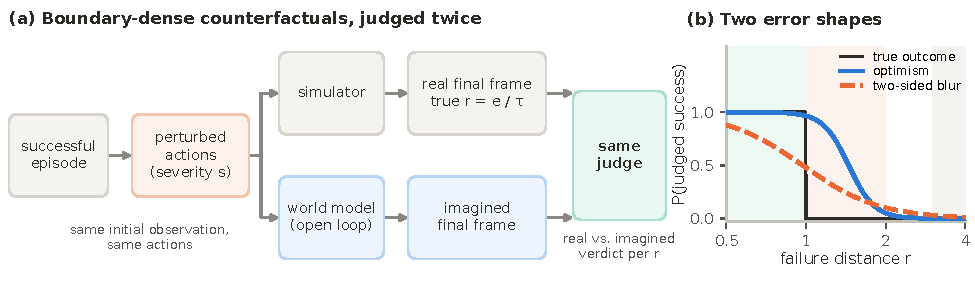
\includegraphics[width=\linewidth]{fig1_protocol.pdf}
\caption{(a) Measurement protocol. A successful episode's actions are perturbed with a severity chosen so that failures fall densely around the success boundary; the simulator gives the true failure distance $r=e/\tau$, and the world model replays the same actions from the same initial observation. One judge scores both final frames, so that its error on the real frame can be subtracted from its error on the imagined frame. (b) Schematic of two ways imagined evaluation can misjudge the outcome step: optimism moves the boundary outward; blur in both directions turns the step into a slope. The shaded bands mark successes ($r<1$), near misses ($1\le r<2$) and far misses ($r\ge3$).}
\label{fig:protocol}
\end{figure}

Our contributions are the protocol (failure-distance curves, paired judging with a perception floor and an imagination share, an imagined-feature probe, and a failure-geometry-weighted rank error, FGRE), its application to three world models with every planned test reported whether or not it held, and the following findings:
\begin{itemize}
\item \textbf{Imagination loses resolution at the boundary (M1).} Five imagination steps ahead, the AUROC for separating successes from near misses falls from 0.953 on real frames to 0.853 in imagination, against far misses by only 0.005, and the near-miss drop grows with every imagination step. A probe trained on imagined features stays below the reference judge on real frames, a sign that part of the boundary information is lost. The errors run in both directions: successes are judged successful less often, near misses only slightly more often, and the net bias is pessimistic. On the PointMaze checkpoint, the near-miss drop (0.197), its growth with the horizon and the information loss recur, but far misses blur as well (0.076).
\item \textbf{Rare training failures make imagination optimistic (M3).} Lowering the training failure rate from 0.3 to 0.03 raises the share of near misses imagined as successful from 0.10 to 0.54 while success misjudgments fall to zero; the judge makes no errors on real frames, so all of this is added by imagination. Here the imagined features keep the information: the error is a shift toward success, whose size also depends on predictor capacity. On M1, a short success-skewed fine-tuning produced only the drop in success misjudgments.
\item \textbf{The judge itself can account for much of the error.} Where the judge errs little on real near misses, imagination adds most of the near-miss errors (shares 0.83 on M2 and 1.00 on M3); on M1 the judge itself labels 0.11 of near misses as successful on real frames, and a vision--language model (VLM) judge labels most of them as successful before imagination is involved.
\item \textbf{Policy-level consequences are bounded, and boundary-targeted training data are no better than reweighting.} In M3 the overestimation that imagination adds follows each policy's near-miss share (Spearman correlation 0.83): a near-failing policy with real success 0.53 is imagined at 0.99, above policies with much higher real success, while a far-failing one with 0.48 is imagined at 0.58. On M1 this overestimation stays within $\pm$0.06 per policy. At matched failure exposure, boundary-targeted counterfactual data were no better than simple reweighting, and a training-free MC dropout discount reduced the bias only slightly.
\end{itemize}

Not every test held: the video world model blurs failures at every distance, so the boundary-specific pattern is not general to world models, and each of the three tests designated as primary held in only one of the models (Table~\ref{tab:tests}).

% =====================================================================================================
\section{Related Work}
\label{sec:related}

\textbf{World models as policy evaluators.} Action-conditioned world models are used to estimate the success of robot policies, to compare checkpoints and to improve policies without hardware rollouts \citep{quevedo2026worldgym, li2025worldeval, guo2026ctrlworld, gao2026dreamdojo, jeon2026roboworld}. Cosmos Policy \citep{kim2026cosmospolicy} also predicts the futures and values of candidate actions for planning, and latent world models such as DINO-WM \citep{zhou2025dinowm} plan in a frozen feature space. Such evaluators are usually validated by the correlation between imagined and real success rates across policies and by rank agreement, the criteria also used for simulation-based evaluation \citep{li2024simpler}. They are not uniformly optimistic: a Veo-based evaluator correlated well with real success rates while predicting lower absolute values \citep{geminirobotics2025veo}. We add a failure-resolved view of where along the failure-distance axis an evaluator errs, and whether the error comes from its judge or from imagination.

\textbf{Imagining success for failures.} Several recent works report that world models trained mostly on successful demonstrations predict success for failed actions \citep{yang2026mirabench, liu2026worldvlaloop, peng2026fact, li2026dreamtrue, tu2026hfwm, wang2026proworld}, and such hallucinations are a concern when policies are optimized inside world models \citep{zhu2026wmpo, chen2026hawmpo, zhou2026wovrplus}. CureWM \citep{xu2026curewm}, the closest to our setting, measures this optimism on counterfactual failures for public Cosmos Policy and Ctrl-World checkpoints and reduces it by fine-tuning on counterfactuals; its severity closest to the success boundary produced too few failures to analyze, and it leaves policy ranking untested. WorldFailBench \citep{zhang2026worldfailbench} finds that world models underestimate how much success drops between neighboring task conditions, which agrees with our observation that imagination blurs success boundaries; it evaluates closed-loop rollouts and does not index errors by failure distance, separate the judge's errors from those of imagination, or relate the bias to a policy's near-miss share. WorldGuide \citep{liu2026worldguide} and AIM \citep{bateman2026aim} argue that successful demonstrations alone do not teach a world model the success boundary or the full influence of actions; our controlled failure-rate sweep tests this data side directly, and our matched-exposure comparison tests the remedy.

\textbf{Judges, ranking metrics and class imbalance.} Judging success from a final frame is itself error-prone: VLM judges lean toward success when a case is ambiguous \citep{navasardyan2026failbench}, distances in a latent space need not track task progress \citep{moukheiber2026tempo}, and failure signals can also be read from a world model's internal states during real execution \citep{pei2026farm}. The mean maximum rank violation (MMRV) of \citet{li2024simpler} weights a rank violation by the real success difference of the violating pair, so violations between policies with similar success cost little; our FGRE instead weights them by how differently the two policies fail. That training with a rare class shifts a learned decision boundary toward that class is a classical observation \citep{cao2019ldam}; our controlled failure-rate sweep shows the analogous effect in imagined outcomes.

% =====================================================================================================
\section{Measuring Boundary Resolution}
\label{sec:method}

\subsection{Imagined evaluation and failure distance}
A world model receives an initial observation $o_0$ and an action sequence $a_{1:T}$ and returns an imagined final observation $\hat o_T$. A judge maps a final observation and a goal to a score, and a fixed threshold turns the score into a verdict $\hat S\in\{0,1\}$. Executing the same actions in the simulator yields the real final observation $o_T$ and the final state, from which the task error $e$ is computed. The failure distance is $r=e/\tau$, where $\tau$ is the task's success threshold, and we use the bins success ($r<1$), near miss ($1\le r<2$), mid ($2\le r<3$) and far miss ($r\ge3$). The primary analyses, however, use the continuous curves $P(\hat S=1\mid r)$ on real and on imagined frames. Throughout, the world model replays the executed actions (open loop), which removes any interaction between the policy and imagined observations and isolates outcome prediction.

\subsection{Paired judging: perception floor and imagination share}
Each counterfactual yields a verdict on the real final frame, $\hat S_{\rm real}$, and on the imagined one, $\hat S_{\rm imag}$, from the same judge. The \emph{perception floor} $F=P(\hat S_{\rm real}=1\mid\text{near miss})$ is the judge's own near-miss error. We call $\mathrm{NM}=P(\hat S_{\rm imag}=1\mid\text{near miss})$ the near-miss misjudgment and $\mathrm{SM}=P(\hat S_{\rm imag}=0\mid r<1)$ the success misjudgment, and define the \emph{imagination share} of near-miss errors as $(\mathrm{NM}-F)/\mathrm{NM}$; where imagination lowers the rate ($\mathrm{NM}<F$) no share is reported.

\subsection{Boundary resolution and the imagined-feature probe}
Boundary resolution is the area under the ROC curve (AUROC) of the judge's score for successes against near misses (the success vs.\ near-miss AUROC) and, separately, against far misses (the success vs.\ far-miss AUROC), on real and on imagined frames. A loss specific to the boundary (boundary specificity) means $\dauc_{\rm near}\ge 0.05$ while $\dauc_{\rm far}\le0.02$, where the drop is $\dauc=\mathrm{AUROC}_{\rm real}-\mathrm{AUROC}_{\rm imag}$. We summarize the trend over horizons by the slope of $\mathrm{AUROC}_{\rm imag}-\mathrm{AUROC}_{\rm real}$ (successes against near misses), the horizon slope; a negative slope means that the drop grows with the horizon. A judge trained on real frames can lose resolution on imagined frames because the imagined features no longer contain the information or because they contain it in a shifted distribution. To separate the two, we train a probe of the same architecture directly on imagined features with the true labels. Its AUROC is a lower bound on the separability that a judge of this class can obtain from imagined features, so a probe that falls well below the reference judge on real frames indicates, but does not prove, that information was lost. We also fit a logistic model in $\log r$ and report $r_{50}$, where the fitted probability of a success verdict on imagined frames crosses 0.5, and the blur width $\Delta r_{10}=r^{\rm imag}_{10}-r^{\rm real}_{10}$, where $r_{10}$ is the distance at which it falls to 0.1.

\subsection{Policy-level quantities}
For a policy $\pi$ evaluated from a fixed set of initial states, let $s_\pi$ be the real success rate, $\hat s_\pi$ the imagined success rate, and $\hat s^{\rm real}_\pi$ the success rate that the same judge assigns to the real final frames. The overestimation $o_\pi=\hat s_\pi-s_\pi$ splits into the part added by imagination, $o^{\rm imag}_\pi=\hat s_\pi-\hat s^{\rm real}_\pi$, and the judge's part, $o^{\rm judge}_\pi=\hat s^{\rm real}_\pi-s_\pi$. The near-miss share $n_\pi$ is the fraction of the policy's episodes with $1\le r<2$. As standard ranking metrics we report the Pearson correlation of $\hat s_\pi$ with $s_\pi$ and the MMRV of \citet{li2024simpler}, which weights each rank violation by the real success difference of the violating pair, so a reversal between two policies with nearly equal real success counts for almost nothing. We therefore also report Kendall's $\tau_b$ computed over the policy pairs with $|s_i-s_j|\le0.05$ (a concordance restricted to similar-success pairs) and a failure-geometry-weighted rank error,
\begin{equation}
\mathrm{FGRE}=\frac1N\sum_{i=1}^{N} \max_{j:\,|s_i-s_j|\le 0.05} |n_i-n_j|\;\mathbb{1}\big[(\hat s_i<\hat s_j)\neq(s_i<s_j)\big],
\end{equation}
which counts rank violations among policies with similar real success, weighted by how differently they fail.

\subsection{Boundary-dense counterfactuals}
Each counterfactual perturbs the actions of a successful episode and is executed in the simulator, which returns the true $r$. Severities are chosen so that the achieved $r$ covers $[0.8,3]$ evenly, with tails below 0.8 and above 3 that anchor the curves; all analyses use the achieved $r$. On M1 we bisect, for each stratified target $r^*$, the magnitude of a fixed perturbation pattern (a constant offset or i.i.d.\ noise on the actions, half each): 3,000 targets in $[0.8,3]$ plus 300 in each tail give 3,600 counterfactuals and over 1,300 near misses per cell, one combination of data split, error definition and horizon (likewise on PointMaze, from 200 validation trajectories). On M2 we combine CureWM's six perturbation families \citep{xu2026curewm} with three of our own aimed at the boundary and select, per task, 500 counterfactuals in $[0.8,3)$ plus 100 successes and up to 100 far misses. On M3 we set $r$ directly on a grid. Evaluation initial states are disjoint from those used for judge training and severity calibration (on M2, the calibration demonstrations are a subset of the judge-training ones).

\subsection{Models, judges and policies}
Table~\ref{tab:setup} summarizes the three models; Appendices~\ref{app:m1}--\ref{app:m3} give the details. M1 predicts frozen DINOv2 patch features \citep{oquab2024dinov2}, starting from one real frame; each imagination step covers five control steps. We use two error definitions for M1: the environment's own $r$, which includes the pusher's position, and an object-pose distance $\rob$ that ignores it. We replicated M1's protocol unchanged on the public DINO-WM PointMaze checkpoint (error: distance from the ball to the goal, $\tau=0.5$; its own five-seed reference judge, held-out accuracy 0.966; Appendix~\ref{app:pm}). M2 is a video world model that also acts and predicts values; we insert counterfactual action chunks into its latent sequence as CureWM does. All of M3's training failures lie at $1\le r<2$. Each model's primary judge (a), which we call the reference judge, is a classifier trained on real final frames with simulator labels. Every reference judge and threshold was fixed before any evaluation set was imagined, and a reference judge was admitted only with a held-out accuracy of at least 0.95 on real frames; M1's is a five-seed ensemble \citep{lakshminarayanan2017deepensembles} because single classifiers moved their operating point between retrainings. Auxiliary judges are a latent goal-distance threshold (b) on M1, the value head (c) on M2, and a VLM (d), Qwen2.5-VL-7B \citep{bai2025qwen25vl}, on both; the VLM's prompts, scoring rule and admission criterion (held-out AUROC of at least 0.80) were fixed before it scored any evaluation frame. M1's policies are Diffusion Policy \citep{chi2023diffusionpolicy} checkpoints from three seeds and eight training stages; the imagined verdict of an episode is obtained by replaying its last $5H$ control steps.

\begin{table}[t]
\caption{The three models. Held-out accuracies are on real frames from initial states not used for training the judge.}
\label{tab:setup}
\centering\small
\setlength{\tabcolsep}{4pt}
\begin{tabular}{>{\raggedright}p{2.3cm}>{\raggedright}p{3.8cm}>{\raggedright}p{3.8cm}>{\raggedright\arraybackslash}p{3.8cm}}
\toprule
 & M1 & M2 & M3 \\
\midrule
World model & public DINO-WM, PushT (replicated on PointMaze) & Cosmos Policy (Cosmos-Predict2 2B), LIBERO-Goal & DINO-WM-style predictor trained from scratch; failure rate $p\in\{0.3,0.1,0.03\}$ \\
Imagination & open loop from one real frame, $H\in\{3,5,7,10\}$ imagination steps & last $k\in\{1,\dots,4\}$ action chunks plus a lift chunk & four autoregressive steps \\
Counterfactuals & 3,600 per cell (horizon $\times$ error definition) from 21 validation trajectories (PointMaze: 200) & 4,184 real--imagined pairs, 6 tasks, 165 initial states & 49 values of $r\in[0.6,3]$ $\times$ 128 scenes $\times$ 3 seeds \\
Reference judge (a) & five-seed ensemble on DINOv2 features of final and goal frames (0.9585; PointMaze 0.966) & ResNet-18 on third-person and wrist frames after the lift (0.974) & classifier on real final-frame tokens (1.000) \\
Policies & 24 Diffusion Policy checkpoints $\times$ 100 episodes & not run & 6 scripted policies $\times$ 1,024 scenes \\
\bottomrule
\end{tabular}
\end{table}

\subsection{Analysis plan and statistics}
\label{sec:prereg}
Before the main runs we fixed, in a design document whose hash and time were logged, the error definitions, the judges and their admission criteria, the policy sets, the counterfactual grids and seeds, the tests of Table~\ref{tab:tests} with their thresholds, and a decision rule for the video world model; later changes were appended as dated amendments, and analyses chosen after seeing results are marked post hoc. Appendix~\ref{app:prereg} gives the record, including which values were already known when a cell was fixed (in particular M3's policy-level values, because M3 reuses the models of a pilot study). The plan designated three tests as primary and specified Holm's method \citep{holm1979simple} for them; because each failed the two-model aggregation rule (held overall only if held in at least two models) before any correction, no correction could change a conclusion (Appendix~\ref{app:tests}). The decision rule was that if neither boundary-specific test held on M2, the claims would be limited to latent world models. Thresholds are applied to point estimates, with 95\% cluster-bootstrap intervals (clusters: source trajectories for M1 and PointMaze counterfactuals, initial states for M1 policies and M2, scenes for M3) and 1,000 to 10,000 resamples. The PointMaze replication was added later as a dated addendum and is not counted in the aggregation (Appendix~\ref{app:prereg}).

\begin{table}[t]
\caption{The tests, with thresholds fixed before the main runs, and their outcomes in the primary cells: for H1 and H3, judge (a), M1 at $H=5$ under the environment's $r$, M2 after one chunk, M3 at $p=0.03$; for H2 and H5b, M1's 24 checkpoints at $H=5$ (near misses on $\rob$) and M3's six policies at $p=0.03$ (near misses on $1\le r<1.2$); for H4 and H5a, the cells of Sections~\ref{sec:skew} and~\ref{sec:remedies}. Appendix~\ref{app:tests} gives intervals. $^a$Fixed imagination length, so the horizon clause cannot be evaluated; the other two clauses hold (0.107 / 0.000). $^b$Judge operating point shifts on imagined frames (Section~\ref{sec:judge}). $^c$Near-miss and horizon clauses hold (0.197; slope $-0.033$); the far-miss clause fails (0.076).}
\label{tab:tests}
\centering\footnotesize
\setlength{\tabcolsep}{3.5pt}
\begin{tabular}{>{\raggedright}p{5.5cm}>{\raggedright}p{2.35cm}>{\raggedright}p{2.35cm}>{\raggedright}p{2.35cm}>{\raggedright\arraybackslash}p{1.45cm}}
\toprule
Test & M1 & M2 & M3 & Overall \\
\midrule
\multicolumn{5}{l}{\emph{Primary tests (multiplicity-corrected)}} \\
H1a: NM $\ge0.3$ and $\ge3\times$ far; decreasing in $r$ & no (0.147) & no (0.298; 2.52$\times$) & \yes{} (0.535; 53.5$\times$) & no \\
H1b: $\dauc_{\rm near}\ge0.05$, $\dauc_{\rm far}\le0.02$, widening with horizon & \yes{} (0.100 / 0.005) & no (0.275 / 0.137) & not counted$^a$ & no \\
H2a: Spearman$(n_\pi,o^{\rm imag}_\pi)\ge0.6$ & no (0.357) & not run & \yes{} (0.829) & no \\
\midrule
\multicolumn{5}{l}{\emph{Other tests}} \\
H2b: a similar-success pair $\ge0.15$ apart; $\tau_b\le0.5$ & no (no pair) & not run & no ($\tau_b$ 1.0) & no \\
H2c: Pearson $\ge0.8$ and MMRV $\le0.05$ & \yes{} & not run & no & per model \\
H3: imagination share of near-miss errors $>0.5$ & no (0.239) & \yes$^b$ (0.829) & \yes{} (1.000) & \yes{} \\
H4a: success skew raises NM, lowers SM & no (NM interval spans 0) & --- & \yes{} & \yes{} \\
H4b: real AUROC $\ge0.95$, probe $\ge0.05$ lower & \yes{} (0.064) & --- & no (0.014) & per model \\
H5a: boundary-targeted data beat (i) and (iv) & no & --- & no (2 settings) & no (0/3) \\
H5b: discount lowers mean $|o_\pi|$ and FGRE & \yes{} & --- & --- & \yes{} \\
H6: checkpoint-selection regret & \multicolumn{4}{l}{not run (dropped after M1's policy-level bias proved small)} \\
\midrule
\multicolumn{5}{l}{\emph{Replication of M1's protocol on a second public DINO-WM checkpoint (PointMaze); not counted above}} \\
H1b, PointMaze & no (0.197 / 0.076)$^c$ & --- & --- & not counted \\
H4b, PointMaze & \yes{} (0.203) & --- & --- & not counted \\
\bottomrule
\end{tabular}
\end{table}

% =====================================================================================================
\section{Imagination Loses Resolution at the Boundary}
\label{sec:boundary}

\begin{figure}[t]
\centering
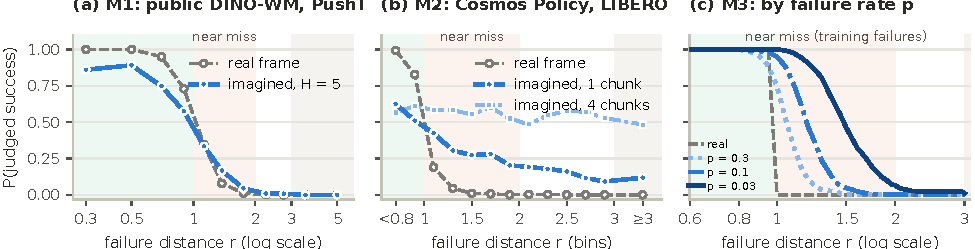
\includegraphics[width=\linewidth]{fig2_curves.pdf}
\caption{Failure-distance curves: share of counterfactuals judged successful by the reference judge (a), on real and on imagined final frames. (a) M1 at $H=5$ (validation split, environment's $r$, binned by $r$). (b) M2, six tasks pooled, after one and after four imagined chunks; the outer bins are $r<0.8$ and $r\ge3$. (c) M3, imagined verdicts for each training failure rate $p$ (three seeds pooled; the primary cell is $p=0.03$) and the real-frame verdict; training failures cover only $1\le r<2$, so the curves beyond $r=2$ are extrapolations. M1 blurs the boundary in both directions, M3 shifts it outward, and M2 degrades over the whole failure range.}
\label{fig:curves}
\end{figure}

\subsection{A public latent world model (M1), on two tasks}
Figure~\ref{fig:curves}a shows M1's failure-distance curve at the primary horizon $H=5$. On real frames the judge labels 0.862 of successes and 0.112 of near misses as successful. In imagination these become 0.710 and 0.147, far misses remain at zero, and among failures the imagined curve still decreases with $r$ (logistic slope in $\log r$: $-5.50$ [$-6.46$, $-4.86$]). The loss of resolution is concentrated at the boundary: the success vs.\ near-miss AUROC falls from 0.953 to 0.853 ($\dauc$ 0.100 [0.075, 0.125]) and the success vs.\ far-miss AUROC by 0.005 [0.001, 0.010]. The near-miss drop grows with the horizon, from 0.053 at $H=3$ through 0.100 and 0.183 to 0.266 at $H=10$; the slope of $\mathrm{AUROC}_{\rm imag}-\mathrm{AUROC}_{\rm real}$ is $-0.031$ [$-0.039$, $-0.025$] per imagination step (Figure~\ref{fig:horizon}a). This is the boundary-specific pattern of Table~\ref{tab:tests} (H1b). Its strong form, in which many near misses are imagined as successes (H1a), does not hold on M1: 0.147 is well below the threshold of 0.3.

The errors run in both directions (Figure~\ref{fig:horizon}c). Imagination moves near misses slightly toward success but successes much more toward failure, so the fitted boundary moves inward ($r_{50}$ from 1.03 to 0.90) while the curve flattens ($\Delta r_{10}$ 0.21 [0.15, 0.28]); the net bias is pessimistic. We therefore describe M1 as losing resolution at the boundary, not as optimistic.

Boundary specificity is limited. Far misses stay separated up to $H=5$ but start to blur at $H=7$ (0.021) and $H=10$ (0.048), and under the object-pose definition $\rob$ they blur at every horizon ($\dauc_{\rm far}$ 0.058--0.129). We therefore restrict the claim of boundary specificity to the environment's $r$ at $H\le5$. Under $r$, the pusher's position dominates the error of 85\% of near misses (1,161 of 1,366), and the perception floor is higher than under $\rob$ (0.112 against 0.047, with a different judge and grid). The same pattern appears on the world model's training-split trajectories (slope $-0.026$ [$-0.030$, $-0.021$]; Appendix~\ref{app:more}).

\textbf{A second public task.} On the DINO-WM PointMaze checkpoint, with the same protocol and a more accurate reference judge (0.966; perception floor 0.047), the loss at the boundary is larger: the success vs.\ near-miss AUROC falls from 0.980 to 0.784 ($\dauc$ 0.197 [0.172, 0.225]), the near-miss misjudgment rises from 0.047 to 0.201 [0.177, 0.227], and the horizon dependence is the same as on PushT (slope $-0.033$ [$-0.037$, $-0.028$]; Figure~\ref{fig:horizon}b). The errors again run in both directions and are net pessimistic (successes judged successful fall from 0.891 to 0.663; $r_{50}$ from 0.99 to 0.85). But far misses blur as well: the success vs.\ far-miss AUROC falls from 1.000 to 0.924 ($\dauc_{\rm far}$ 0.076 [0.057, 0.097]) and by 0.241 at $H=10$, and no cell meets the 0.02 bound, so the far-miss clause of the boundary-specific test fails (Table~\ref{tab:tests}; Appendix~\ref{app:pm}). Across the two tasks the loss starts at the boundary and spreads outward with the horizon (blur width $\Delta r_{10}$ from 0.15 to 0.47 on PushT and from 0.50 to 2.19 on PointMaze between $H=3$ and $H=10$). Strict boundary specificity thus holds only on PushT under $r$ at $H\le5$; both tasks share a near-miss drop several times the far-miss drop (2.6$\times$ at $H=5$ on PointMaze) that grows with the horizon.

\begin{figure}[t]
\centering
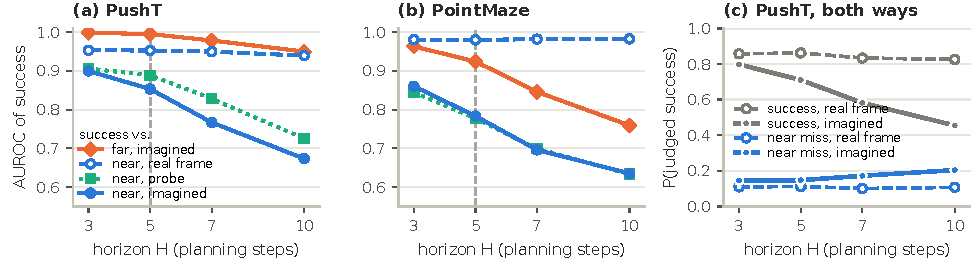
\includegraphics[width=\linewidth]{fig3_m1_horizon.pdf}
\caption{The two public DINO-WM checkpoints by imagination horizon (validation split, judge (a); PushT under the environment's $r$). (a) PushT and (b) PointMaze: success vs.\ near-miss AUROC on real frames, on imagined frames and for a probe trained on imagined features, and success vs.\ far-miss AUROC on imagined frames; dashed vertical line: the primary cell $H=5$. (c) PushT: share judged successful among successes and among near misses; imagination moves both, in opposite directions.}
\label{fig:horizon}
\end{figure}

\subsection{A controlled latent world model (M3)}
M3's reference judge makes no errors on real final frames (perception floor 0.000). At $p=0.03$, imagination judges 0.535 [0.503, 0.566] of near misses successful, and 0.979 of those with $1\le r<1.2$; far misses at $r=3$ are almost never judged successful (0.010 [0.000, 0.023]) and successes always are (Figure~\ref{fig:curves}c). The success vs.\ near-miss AUROC falls from 1.000 to 0.893 ($\dauc$ 0.107 [0.095, 0.119]), and the success vs.\ far-miss AUROC does not fall at all. Here the strong form holds (H1a: near/far ratio 53.5 [23.3, 170]), and so do the two AUROC clauses of the boundary-specific test; its horizon clause cannot be tested with M3's fixed four-step imagination (Table~\ref{tab:tests}). Unlike M1's, M3's imagined boundary moves outward ($r_{50}$ 1.51 [1.47, 1.54]; $\Delta r_{10}$ 0.95 [0.86, 1.03]), the optimistic shape of Figure~\ref{fig:protocol}b.

\subsection{A video world model (M2)}
\label{sec:m2}
Cosmos Policy's imagination degrades over the whole failure range rather than at the boundary (Figure~\ref{fig:curves}b). With the reference judge, the near-miss misjudgment rises from 0.051 on real frames to 0.298 [0.241, 0.355] after one imagined chunk, but far misses are also judged successful (0.118 [0.071, 0.170]; ratio 2.52 [1.79, 3.95]). The success vs.\ near-miss AUROC drops by 0.275 [0.240, 0.311] and the success vs.\ far-miss AUROC by 0.137 [0.104, 0.173], above the bound of 0.02. Both drops grow as chunks are chained, the far-miss drop faster (slopes of $\mathrm{AUROC}_{\rm imag}-\mathrm{AUROC}_{\rm real}$: $-0.104$ against $-0.065$ [$-0.077$, $-0.052$] per chunk), and after four chunks the imagined verdict is close to chance (AUROC 0.511 against near misses and 0.561 against far misses). Neither boundary-specific test holds (Table~\ref{tab:tests}); following the decision rule fixed for this case, we limit our claims to latent world models, and we did not run M2's policy-level stage. Post-hoc observations do not change this: the near-miss misjudgment and the ratio lie just below their thresholds; most far misses judged successful come from one task (0.680 of its far misses; Appendix~\ref{app:m2}); and a linear probe on DINOv2 features of the imagined frames, which loses less against far misses than the judge (0.036 against 0.137 after one chunk), still exceeds 0.02 and reaches 0.110 after two chunks.

% =====================================================================================================
\section{Where the Error Enters}
\label{sec:source}

\begin{figure}[t]
\centering
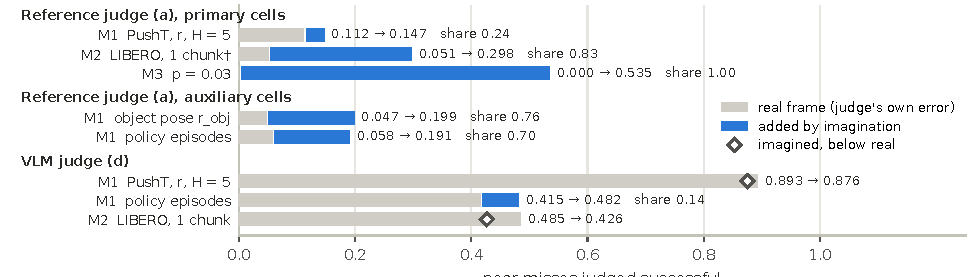
\includegraphics[width=\linewidth]{fig4_decomp.pdf}
\caption{Near-miss misjudgment split into the judge's own error on real frames (gray) and the part added by imagination (blue), with the imagination share. Top: the primary cells of H3. Middle: M1 under the object-pose distance and on Diffusion Policy episodes. Bottom: the VLM judge, which errs mostly on real frames; a diamond marks an imagined rate below the real-frame rate. $^\dagger$M2's judge shifts its operating point on imagined frames, so part of its share may be a judge domain gap.}
\label{fig:decomp}
\end{figure}

\subsection{Judge versus imagination}
\label{sec:judge}
Figure~\ref{fig:decomp} splits near-miss misjudgments into the judge's own error on real frames and the part that imagination adds. In the primary cells the imagination share is 0.829 [0.754, 0.886] on M2 and 1.000 on M3 (H3 in Table~\ref{tab:tests}); on M1 it is 0.239 [0.067, 0.389], because its judge already labels 0.112 of near misses as successful on real frames. Under $\rob$ and on policy episodes, where M1's perception floor is lower (0.047 and 0.058), its share is 0.765 and 0.698; on PointMaze (floor 0.047) it is 0.766. M2 needs a caveat. Its judge was trained on real post-lift frames, and on imagined frames its operating point moves: it labels 0.938 of successes as successful on real frames but 0.588 on imagined ones, with large differences between tasks. In imagination the arm does not rise as far during the lift, which changes the wrist view (Appendix~\ref{app:m2}, Figure~\ref{fig:frames}); part of M2's imagination share may therefore be a judge domain gap.

Off-the-shelf judges can account for most of the error themselves. The VLM judge, shown the goal and the final frame, labels 0.893 of M1's near misses as successful already on real frames (0.671 under $\rob$), 0.415 on policy episodes and 0.485 on M2; imagination adds little or nothing (Figure~\ref{fig:decomp}). The VLM met its admission criterion only on policy episodes, where the target outline is visible (0.909; 0.614 and 0.682 on M1's goal-image sets, below 0.80 on M2). Cosmos Policy's value head similarly judges 0.760 of near misses successful from real end states, and in our reproduction of CureWM's branch-point measurement (optimism, the share of counterfactual failures predicted as successes: 79.4\% in our run, 79.13\% reported) the optimism was unchanged when the value head saw real future frames (79.8\%): there, it comes from the value head, not from imagination.

\subsection{Information loss versus distribution shift}
\label{sec:infoloss}
The imagined-feature probe distinguishes the two latent world models (H4b). On M1, a probe trained on imagined features reaches 0.889, against 0.953 for the judge on real frames (gap 0.064 [0.046, 0.084]), and the gap widens with the horizon (0.047 at $H=3$, 0.121 at $H=7$, 0.214 at $H=10$): imagined features keep less boundary information than the same architecture extracts from real frames, and less at longer horizons, so H4b holds on M1. The PointMaze loss is almost entirely of this kind: the probe reaches 0.778 against 0.980 on real frames (gap 0.203) and tracks the reference judge's imagined-frame AUROC within 0.02 at every horizon, so a judge fitted to imagined features would recover little. M3's probe reaches 0.986 against 1.000 (gap 0.014 [0.011, 0.016]), so H4b fails there: the imagined features still separate near misses, and the reference judge errs because the imagined distribution has shifted toward success.

% =====================================================================================================
\section{Rare Training Failures Make Imagination Optimistic}
\label{sec:skew}

Varying M3's training failure rate shows what drives the shift of Section~\ref{sec:infoloss} (Figure~\ref{fig:curves}c; H4a in Table~\ref{tab:tests}). As $p$ falls from 0.3 to 0.1 to 0.03, the near-miss misjudgment rises from 0.104 to 0.238 to 0.535 while the success misjudgment falls from 0.0215 to 0.0046 to 0.000 ($p=0.03$ against 0.3: $+0.431$ [0.406, 0.457] and $-0.0215$ [$-0.030$, $-0.014$]); both adjacent steps are significant (bootstrap intervals exclude zero), and the imagined boundary $r_{50}$ moves from 1.06 to 1.20 to 1.51. Since the judge makes no errors on real frames, the whole change happens in imagination. In M3, success-skewed training data thus shift the imagined boundary outward with the skew.

On M1, only one of the two predicted effects appeared. We fine-tuned M1's predictor for 3,000 steps on 10,000 windows that were 97\% or 50\% successes, drawn as nested subsets of one pool. The success-skewed model misjudged fewer successes ($-0.029$ [$-0.053$, $-0.006$]) but not more near misses under $r$ ($+0.007$ [$-0.006$, 0.019], an interval that includes zero); under $\rob$ both effects appeared ($+0.019$ [0.006, 0.031] and $-0.037$ [$-0.054$, $-0.021$]). We cannot tell whether the null result under $r$ reflects no effect or too short a fine-tuning.

\textbf{Predictor capacity (a descriptive analysis, not a planned test).} In M3, predictor capacity sets how far the imagined distribution shifts (Table~\ref{tab:capacity} in Appendix~\ref{app:more}). With a smaller predictor every near miss is imagined as a success (NM 1.000); with a larger one NM falls to 0.149 and the reference judge's AUROC rises to 0.956, while the probe stays between 0.967 and 0.993 in every variant except the 384-dimensional one (0.899). Using four times as many tokens did not help (NM 0.614). Keeping 384 PCA dimensions per token made training harder under per-dimension normalization and produced blur in both directions (SM 0.264), which we do not attribute to the representation itself. The variables that decide the outcome also carry little of the training signal (Appendix~\ref{app:more}), and a loss that up-weighted them did not help (Section~\ref{sec:remedies}).

% =====================================================================================================
\section{Consequences for Policy Evaluation}
\label{sec:policy}

In M3 the bias follows how policies fail (Figure~\ref{fig:policy}a). With $p=0.03$, the overestimation added by imagination follows the near-miss share: the Spearman correlation between $n_\pi$ and $o^{\rm imag}_\pi$ is 0.829 [0.771, 0.943] (exact one-sided permutation test, $P=0.029$), above the threshold of 0.6 (H2a in Table~\ref{tab:tests}; the pilot had shown this with the same models, Appendix~\ref{app:prereg}). A policy that fails just beyond the boundary ($\pi_6$, real success 0.526) is imagined at 0.985, one that fails farther away ($\pi_5$, 0.482) at 0.580, and one with widely spread errors ($\pi_4$, 0.521) at 0.722. With the designed band $1\le r<2$, which also counts $\pi_5$'s failures as near misses, the correlation is 0.66. Among these three policies with similar real success the imagined order matches the real one ($\tau_b=1.0$ over their pairs) even though they are imagined far apart (H2b). The overestimation does reorder policies whose real success differs: the near-failer is imagined above $\pi_3$ (real 0.716, imagined 0.886) and narrowly above $\pi_2$ (real 0.901, imagined 0.982). The standard metrics register this (Pearson correlation 0.694, MMRV 0.157; H2c). This policy-level result largely follows from the curve: $\pi_6$'s failures lie at $1\le r<1.2$, where 0.979 of near misses are imagined as successes.

On M1 the bias stays small (Figure~\ref{fig:policy}b). Over the 24 Diffusion Policy checkpoints, imagination raises the share of near-miss episodes judged successful from 0.058 to 0.191, but near misses make up only 0.02 to 0.28 of a policy's episodes, so $o^{\rm imag}_\pi$ stays between $-$0.01 and $+$0.06. The Spearman correlation between $n_\pi$ and $o^{\rm imag}_\pi$ is 0.357 [0.023, 0.598] (one-sided Monte Carlo permutation test, $P=0.047$), below the threshold of 0.6. No pair of checkpoints within 0.05 in real success is imagined 0.15 apart (the largest imagined difference among the 43 such pairs is 0.060). The standard metrics agree closely with the real ranking (Pearson correlation 0.998, MMRV 0.010; H2c), but as there is no reversal for them to miss, we do not take this as evidence that they hide one.

On a control set of eight hand-designed perturbation policies on M1 in two clusters of similar success, the imagined order of the 12 similar-success pairs agrees with the real one no better than chance ($\tau_b=0.000$), and FGRE is 0.117 while MMRV is 0.023 (Table~\ref{tab:rank}): FGRE targets such reversals between policies that fail differently. It is not a general bias measure: on M3 it is 0.000 despite the large bias, because no similar pair is reversed. The judge matters at the policy level as well: with the VLM judge on M1's checkpoints, two checkpoints with equal real success (0.74) are imagined at 0.83 and 0.67, and MMRV rises to 0.067.

\begin{figure}[t]
\centering
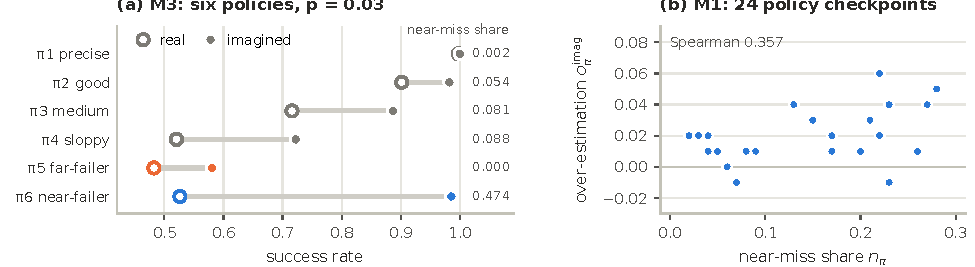
\includegraphics[width=\linewidth]{fig6_policy.pdf}
\caption{Policy-level overestimation. (a) M3 at $p=0.03$: real (open) and imagined (filled) success of six scripted policies; right column: near-miss share on $1\le r<1.2$. The near-failer $\pi_6$ and the far-failer $\pi_5$ have similar real success. (b) M1: overestimation added by imagination against the near-miss share ($1\le\rob<2$) for 24 Diffusion Policy checkpoints at $H=5$.}
\label{fig:policy}
\end{figure}

% =====================================================================================================
\section{Remedies}
\label{sec:remedies}

\textbf{Data side, at matched exposure (H5a).} We compared five ways of using a fixed number of unique failures (300 on M1; the default training failures on M3) at the same 25\% share of failures per batch, by fine-tuning M1 for 3,000 steps or training M3 from scratch (Table~\ref{tab:remedies}): (i) uniform reweighting; (ii) counterfactuals at the boundary ($1\le r<2$ on M1, $1\le r<1.2$ on M3); (iii) (ii) with a matched success just inside it; (iv) full-range counterfactuals as in CureWM ($1\le r\le6$ on M1, $1\le r\le3$ on M3); (v) (i) with a loss that up-weights the object's patches. On M3, where every training failure already lies at $1\le r<2$, (i) reweights these failures and (ii)--(iv) redraw the same failure scenes at other distances. We had predicted that (ii) would beat both (i) and (iv) in at least two of the three settings (H5a); it did so in none. On M1, (ii) matched reweighting ($+0.001$ [$-0.011$, 0.014]) although it beat full-range counterfactuals ($-0.012$ [$-0.021$, $-0.003$]); on M3 boundary-targeted data were worse than reweighting by 0.040 [0.017, 0.064] at $p=0.03$ and by 0.046 [0.028, 0.065] at $p=0.1$, and in a post-hoc check on $1\le r<1.2$, the band that (ii) targets, it still did not beat reweighting (0.721 against 0.699 at $p=0.03$). This contradicts our pilot's interpretation, which had not matched exposure. On M3, failure exposure itself reduced NM (not a planned test): every variant, plain reweighting included, cut NM from 0.535 to between 0.187 and 0.227 at $p=0.03$, at a cost of at most 0.016 in SM. M1's 3,000 fine-tuning steps moved NM by about 0.01 at most, and the boundary-weighted loss (v) matched reweighting on both models.

\begin{table}[t]
\caption{Data-side remedies at matched failure exposure: NM / SM for each training variant (H5a). (0) no remedy (M1: success-skewed fine-tuning; M3: default training); (i) uniform reweighting; (ii) boundary-targeted counterfactuals; (iii) contrast pairs; (iv) full-range counterfactuals; (v) reweighting plus a boundary-weighted loss. Last column: NM of (ii) minus (i) with a 95\% paired cluster-bootstrap interval (clusters as in Section~\ref{sec:prereg}). Three seeds per variant.}
\label{tab:remedies}
\centering\footnotesize
\setlength{\tabcolsep}{2.6pt}
\begin{tabular}{lccccccc}
\toprule
Setting & (0) & (i) & (ii) & (iii) & (iv) & (v) & NM: (ii) $-$ (i) \\
\midrule
\inputrows{tables/tab_remedies.tex}
\bottomrule
\end{tabular}
\end{table}

\textbf{Evaluation side (H5b).} Without retraining, we ran M1 with its predictor's dropout active at inference (MC dropout) \citep{gal2016dropout}, imagined each window 16 times and counted the window as successful only if at least $q^*$ of its 16 verdicts were successes, with $q^*=13/16$ chosen on separate development episodes. Mean $|o_\pi|$ fell from 0.0233 to 0.0187 ($-0.0046$ [$-0.0088$, $-0.0004$]) and FGRE from 0.0225 to 0.0171, and the dependence of the overestimation on the near-miss share disappeared (Spearman correlation 0.357 to 0.020; H5b). The gain is small because M1's policy-level bias is already small, and it depends on the agreement threshold: a simple majority over the 16 samples made the bias worse (0.0283).

% =====================================================================================================
\section{Discussion and Limitations}
\label{sec:discussion}

\textbf{Two mechanisms.} On both public DINO-WM checkpoints, imagined features separate near misses less well than real ones, increasingly over longer horizons, and the errors run in both directions; in M3 the features keep the information but shift toward the outcome that dominates training, more so as failures become rarer (and, in a descriptive sweep, as the predictor shrinks). The first calls for better predictors or shorter horizons; the second suggests that failure exposure, or a judge fitted to imagined features, could recover much of the boundary, which we did not test.

\textbf{Implications for imagined evaluation.} (1) Report boundary-resolved diagnostics, such as failure-distance curves and the success vs.\ near-miss and success vs.\ far-miss AUROC, alongside correlations of success rates, because they show which failures are misjudged. On M1, near misses were rare, so imagination changed policy-level estimates by at most 0.06. (2) Score real final frames with the same judge, because the judge itself can account for most of the error (the VLM and the value head here). (3) In our controlled model, success-skewed training data and a smaller predictor both produced optimism; more failure exposure reduced it, and placing the failures at the boundary added nothing. (4) Compare policies that fail in different ways with care: in M3 the near-failer with real success 0.526 was imagined at 0.985, above policies with much higher real success, and the far-failer with similar real success was not.

\textbf{Limitations.} Our claims rest on two latent world models, and on different parts of them: information loss (H4b) was shown on the public DINO-WM checkpoints only (PushT and PointMaze), optimism and the policy-level relation on M3 only, whose policy-level result was known from a pilot, and strict boundary specificity on PushT only; the only video world model, M2, failed the decision rule, so whether near-miss blindness appears in video world models under other queries remains open. All imagined verdicts replay executed actions (on M1, only the last $5H$ control steps of an episode); we did not test closed-loop imagined evaluation, in which the policy acts on imagined observations. All experiments are simulated, with deterministic failures, and on PushT the environment's distance is dominated by the pusher's position. Reference judges see imagined frames that lie outside their training distribution, which matters most for M2; M1's ensemble passed the admission criterion overall (0.9585) but reached only 0.941 at $H=7$, and policy-level results changed with the judge. M1's counterfactuals come from 21 validation trajectories, the bootstrap clusters, so its intervals are wide. M3's training failures cover only $1\le r<2$, its far-miss bin is a single value ($r=3$), its imagination length is fixed, and its six policies allow only coarse permutation tests. M1's fine-tuning was short, and the MC dropout threshold was chosen on other episodes of the same checkpoints. Several test cells were fixed with partial knowledge of the data, the analysis plan was internal rather than registered externally (Appendix~\ref{app:prereg}), and no primary test held in more than one model.

% =====================================================================================================
\section{Conclusion}
\label{sec:conclusion}

On a public latent world model, on two tasks, imagination loses resolution at the success boundary, and more at longer horizons, with errors in both directions and some information lost; on one task the loss stays confined to the boundary, on the other it spreads to far misses. In a controlled latent world model the imagined features keep that information but shift toward success, increasingly as training failures become rarer, and the overestimation that imagination adds then tracks how often a policy fails narrowly. When the judge itself erred little on real near misses, most near-miss errors were added by imagination. At matched failure exposure, placing training failures at the boundary did not beat reweighting them. The video world model we tested failed in a different way, one not specific to the boundary. The protocol requires only a simulator that executes perturbed actions and a judge applied to both real and imagined frames.

\section*{Broader Impact Statement}
Our results suggest that imagined policy evaluation can be least reliable for policies that fail narrowly, and that judges such as VLMs or value heads can add optimism of their own. Over-trusting such evaluations could let unsafe policies pass; we hope that boundary-resolved reporting reduces this risk. We do not see a direct negative societal impact of this work.

\bibliography{refs}
\bibliographystyle{tmlr}

% =====================================================================================================
\clearpage
\appendix

\section{Analysis Plan Record}
\label{app:prereg}

The analysis plan was written before the main runs and frozen as a design document whose SHA-256 hash and time (UTC) were recorded in a run log; later changes were appended as dated sections and never edited in place. Table~\ref{tab:prereg} lists the versions and what was known when each was made. No threshold changed after the freeze, but some cells and rules were fixed with partial knowledge of the data. The main case is M3, which reuses the scene, models and policy set of a pilot study that our reproduction matched bit for bit before the design was written, so its policy-level values were known: M3's H2a confirms the pilot rather than testing a new prediction, whereas its curve grid is new. Its near-miss band for H2a ($1\le r<1.2$, the pilot's band) was also set after the reproduction, because M3's far-failing policy fails at $1.5\le r<2$; the designed band is reported too. The H1 aggregation rule (v2.1) was fixed after M1's and M3's results were known but before M2's; counting M3 on its two evaluable clauses would have made H1b hold in two models, so the rule we fixed is the conservative one. Three amendments followed test outcomes: applying the decision rule for M2 (and dropping H6), fixing how results are described, and computing a pre-defined cell that the stage analysis had omitted. The PointMaze replication (\S12 of the design document) was added after all test outcomes and a first draft of this paper; its cell, judge rules, two tests and stopping rules were fixed before any PointMaze evaluation set was imagined, and its outcome does not enter the aggregation. The current document has the last logged hash. For double-blind review, the supplementary copies of the design document, run log and stage reports are redacted (server names and local paths), so their hashes differ from the logged ones; the unredacted originals will be released with the de-anonymized version. The documents are written in Korean; Section~\ref{sec:method} and Appendices~\ref{app:prereg} and~\ref{app:tests} give their content in English. Five small pilot studies, each with its own plan written before it ran, preceded the design; two of them were extended into M1 and M3, and the M3 pilot also motivated the boundary-targeted remedy that H5a tested.

\begin{table}[h]
\caption{Versions of the design document. Each hash is the first 12 hexadecimal digits of the SHA-256 of the whole document at that time.}
\label{tab:prereg}
\centering\small
\setlength{\tabcolsep}{4pt}
\begin{tabular}{>{\raggedright}p{1.15cm}>{\raggedright}p{2.15cm}>{\raggedright}p{2.3cm}>{\raggedright}p{4.85cm}>{\raggedright\arraybackslash}p{3.65cm}}
\toprule
Version & Time (UTC) & SHA-256 & What it fixed & When, and what was known \\
\midrule
v1 & 2026-10-21 21:07 & 6e131532257f & hypotheses, metrics, thresholds, decision rules; error definitions, judges and admission criteria, policy sets, counterfactual grids, splits and seeds for M1--M3 & before the main runs; the pilots had been reproduced, so M3's policy-level values were known \\
v1.1 & 2026-10-21 21:11 & a9fd3c34a8d0 & the primary cell of each model for H1 & before any evaluation set was imagined \\
v2 & 2026-10-21 22:54 & f77fe3dc5fa2 & near-miss band of M3's H2a: $1\le r<1.2$ (designed band also reported) & before M3's policy analysis, with the pilot's policy results known \\
v2.1 & 2026-10-21 23:40 & fd3cfb181ea6 & H1 aggregation counts only models in which every clause can be evaluated; boundary specificity is reported per cell & after M1's and M3's curves, before M2's \\
v2.2 & 2026-10-21 23:49 & 0d22c0d2c5d3 & FGRE and $\tau_b$; H2 cells; H3 cell = H1 cell; VLM procedure & before policy-level and VLM analyses; M1's H3 value was known \\
v3 & 2026-10-22 03:52 & 5b95df58c9d2 & decision rule applied after M2 failed H1a and H1b: claims narrowed to M1 and M3; M2's policy stage and H6 dropped & after M2's outcome (applies the v1 rule; dropping H6 was a new decision) \\
v3.1 & 2026-10-22 04:01 & 570fe107bbb3 & operational definitions for H4 and H5 (NM, SM, fine-tuning data, remedies at matched exposure, H5b rule) & before evaluating H4 and H5; M3's misjudgments by $p$ and both probes were known from the curve stage \\
v3.2 & 2026-10-22 12:00 & 8cf97a97d01b & how H4a, H5a, H5b and the capacity sweep are described & after all test outcomes (outcomes unchanged) \\
\S11 & 2026-10-22 12:55 & ea176a5ce46d & M2's H3 cell, defined in v2.2 but not computed by the stage analysis, computed as defined & after the other outcomes (definition unchanged) \\
\S12 & 2026-10-31 11:13 & 3273f801e657 & replication of M1's protocol on PointMaze: cell, judge rules, tests H1b and H4b with M1's thresholds, stopping rules; not counted in the aggregation & after all test outcomes and a first draft of this paper; before any PointMaze evaluation set was imagined \\
\bottomrule
\end{tabular}
\end{table}

\textbf{Deviations.} All were recorded when they occurred, and none changed a test outcome. (1) M1's policy-level test uses 24 trained checkpoints (power about 0.89 at $\alpha=0.05$ to reject a zero correlation when the true Spearman correlation is 0.6, by the Fisher $z$ approximation) instead of the 32 policies in the design, with the eight hand-designed perturbation policies kept as a separate control. (2) Diffusion Policy was trained for 1,000 instead of 5,000 epochs, and its eight stages were chosen from simulator results only. (3) M1's reference judge became a five-seed ensemble because single retrainings moved the operating point (imagined near-miss misjudgment 0.18 to 0.26 between retrainings, with AUROC stable to $\pm$0.003). (4) A source of randomness in LIBERO fixture placement was found during M2's preparation and fixed by seeding and synchronizing the rendered scene; earlier judge results were discarded. (5) M2's reference judge passed the admission criterion on its pre-specified final attempt and was rebuilt with the same code before the main run. (6) The VLM fell below the admission criterion on M2 and on M1's goal-image sets and was used only as an auxiliary judge there. (7) M2's evaluation set has 4,652 pairs (4,184 on the six tasks with a reference judge plus 468 on the drawer task) instead of 4,900, because two candidate pools were smaller than planned. (8) Two M1 cells were rerun after a seed overflow; replaying policy windows in a separate process differed from the recorded final states by at most 0.0041 pixels and changed no bin. (9) A verdict counted as success when the ensemble probability exceeded 0.5 (the design said at least 0.5; no value equals 0.5). (10) M1 fine-tuning used bfloat16 mixed precision (autocast) in the forward pass, decided before any result. (11) One M3 remedy model was lost to an accidental process kill and retrained with the same seed. (12) Re-running imagination with the original M1 model in batches of a different size changed probabilities by at most 0.016 and no test outcome. (13) Curve summaries use a pooled logistic regression with cluster-bootstrap intervals; the random-intercept logistic model named in the design (one intercept per initial state) gives nearly the same boundary ($r_{50}$ 1.02 on real frames and 0.89 in imagination at $H=5$). (14) Small infrastructure changes: M2 used a byte-identical public copy of a gated autoencoder, a one-step offset in CureWM's branch-point code was kept for the reproduction and corrected in our own queries, and Diffusion Policy's demonstrations came from a mirror verified identical to the original. (15) PointMaze: the severity grid's upper end was used in every cell and 1--38 far-tail targets per cell were dropped as unreachable; a unit conversion left over from PushT mis-scaled a recorded calibration table only (recomputed with the same result); and the stage ran on a rented GPU (Appendix~\ref{app:pm}).

\section{All Planned Tests}
\label{app:tests}

Table~\ref{tab:alltests} gives the values behind Table~\ref{tab:tests}. Threshold conditions are judged on point estimates. Holm's method could not change any conclusion for the three primary tests, because each already fails the two-model aggregation rule of the plan; the bootstrap $P$-values of the interval conditions of H1 are below 0.001, and the one-sided permutation $P$-values of H2a (0.047 on M1, Monte Carlo; 0.029 on M3, exact) are uncorrected.

\begin{table}[h]
\caption{All planned tests with 95\% cluster-bootstrap intervals.}
\label{tab:alltests}
\centering\scriptsize
\setlength{\tabcolsep}{3pt}
\begin{tabular}{>{\raggedright}p{1.0cm}>{\raggedright}p{1.3cm}>{\raggedright}p{1.1cm}>{\raggedright\arraybackslash}p{10.75cm}}
\toprule
Test & Model & Outcome & Values \\
\midrule
H1a & M1 & no & NM 0.147 [0.129, 0.168] (perception floor 0.112); far 0.000; slope in $\log r$ $-5.50$ [$-6.46$, $-4.86$] \\
 & M2 & no & NM 0.298 [0.241, 0.355]; far 0.118 [0.071, 0.170]; ratio 2.52 [1.79, 3.95]; slope $-1.44$ [$-1.82$, $-1.12$] \\
 & M3 & yes & NM 0.535 [0.503, 0.566] (floor 0.000); far 0.010 [0.000, 0.023]; ratio 53.5 [23.3, 170]; slope $-8.69$ [$-9.88$, $-7.76$] \\
H1b & M1 & yes & $\dauc_{\rm near}$ 0.100 [0.075, 0.125]; $\dauc_{\rm far}$ 0.005 [0.001, 0.010]; horizon slope $-0.031$ [$-0.039$, $-0.025$] \\
 & M2 & no & $\dauc_{\rm near}$ 0.275 [0.240, 0.311]; $\dauc_{\rm far}$ 0.137 [0.104, 0.173]; chunk slope $-0.065$ [$-0.077$, $-0.052$] \\
 & M3 & n/a & $\dauc_{\rm near}$ 0.107 [0.095, 0.119]; $\dauc_{\rm far}$ 0.000; horizon fixed \\
 & PointMaze & no & $\dauc_{\rm near}$ 0.197 [0.172, 0.225]; $\dauc_{\rm far}$ 0.076 [0.057, 0.097]; horizon slope $-0.033$ [$-0.037$, $-0.028$] (replication, not counted) \\
H2a & M1 & no & Spearman correlation 0.357 [0.023, 0.598], one-sided Monte Carlo permutation $P$ 0.047 \\
 & M3 & yes & Spearman correlation 0.829 [0.771, 0.943], exact one-sided permutation $P$ 0.029; designed band $1\le r<2$: 0.66 \\
H2b & M1 & no & no qualifying pair (largest imagined difference 0.060 among 43 similar pairs); $\tau_b$ 0.709 [0.286, 0.822] \\
 & M3 & no & two qualifying pairs, but $\tau_b$ 1.0 [$-1.0$, 1.0] (order of the similar policies preserved) \\
H2c & M1 & yes & Pearson correlation 0.998 [0.992, 0.998]; MMRV 0.010 [0.005, 0.028]; FGRE 0.023 [0.014, 0.066] \\
 & M3 & no & Pearson correlation 0.694 [0.649, 0.734]; MMRV 0.157 [0.056, 0.176]; FGRE 0.000 \\
H3 & M1 & no & 0.112 $\to$ 0.147, share 0.239 [0.067, 0.389] \\
 & M2 & yes & 0.051 $\to$ 0.298, share 0.829 [0.754, 0.886] (judge caveat, Section~\ref{sec:judge}) \\
 & M3 & yes & 0.000 $\to$ 0.535, share 1.000 [1.000, 1.000] \\
H4a & M1 & no & 97\% vs.\ 50\% successes: NM $+0.007$ [$-0.006$, 0.019]; SM $-0.029$ [$-0.053$, $-0.006$] \\
 & M3 & yes & $p=0.03$ vs.\ 0.3: NM $+0.431$ [0.406, 0.457]; SM $-0.0215$ [$-0.030$, $-0.014$] \\
H4b & M1 & yes & real 0.953, imagined-feature probe 0.889, gap 0.064 [0.046, 0.084] \\
 & M3 & no & real 1.000, probe 0.986, gap 0.014 [0.011, 0.016] \\
 & PointMaze & yes & real 0.980, probe 0.778, gap 0.203 (replication, not counted) \\
H5a & M1 & no & (ii)$-$(i) $+0.001$ [$-0.011$, 0.014]; (ii)$-$(iv) $-0.012$ [$-0.021$, $-0.003$] \\
 & M3, 0.03 & no & (ii)$-$(i) $+0.040$ [0.017, 0.064]; (ii)$-$(iv) $+0.017$ [$-0.007$, 0.040] \\
 & M3, 0.1 & no & (ii)$-$(i) $+0.046$ [0.028, 0.065]; (ii)$-$(iv) $+0.029$ [0.010, 0.049] \\
H5b & M1 & yes & mean $|o_\pi|$ 0.0233 $\to$ 0.0187, difference $-0.0046$ [$-0.0088$, $-0.0004$]; FGRE 0.0225 $\to$ 0.0171 \\
\bottomrule
\end{tabular}
\end{table}

\section{M1 Details}
\label{app:m1}

\textbf{World model and error definitions.} We use the public DINO-WM PushT checkpoint unchanged. One imagination step covers five control steps; we start from one real frame with proprioception and replay the recorded actions, normalized as in DINO-WM. The goal is the outcome state of the unperturbed expert segment. The environment's error is $r=\max(d_{\rm pos}/20\,\text{pixels},\ |\Delta\theta|/(\pi/9))$, where $d_{\rm pos}$ is the Euclidean norm of the joint difference in pusher and block positions and $\Delta\theta$ the block's angle difference, so $r<1$ coincides with the environment's success check; $\rob$ uses the block position only. Episodes of the standard PushT task have no pusher target, so policy episodes use $\rob$ with the fixed goal pose.

\textbf{Splits.} Training-split trajectories of at least 52 steps (18,584) were divided into disjoint sets for judge training (2,000), severity calibration (1,000) and the training-split evaluation set (3,000); the 21 validation trajectories form the main evaluation set. Fine-tuning data (Section~\ref{sec:skew}) came from the remaining training-split trajectories.

\textbf{Counterfactuals.} A counterfactual adds a severity times a fixed pattern to the actions of an expert segment: either a constant offset in a random direction or i.i.d.\ Gaussian noise. For each stratified target $r^*$ the severity is found by 14 steps of bisection; the median $|r-r^*|$ is at most 0.0027 in every cell. Each episode carries six targets and the expert sequence; unreached targets are redrawn.

\textbf{Judges.} Judge (a) takes DINOv2 patch tokens of the final frame $z$ and of the goal $z_g$, forms tokens $[z, z_g, z-z_g]$, and applies a two-layer transformer of width 128 with a class token, trained with a class-balanced cross-entropy and an auxiliary regression of $\log r$. It was trained on 16,000 trajectories (500 episodes $\times$ expert plus seven perturbations $\times$ four horizons), with 20\% of episodes held out. The held-out episodes that decided admission were also used to select the training epoch, so the admission accuracies are slightly upward-biased. We trained separate ensembles for $r$, $\rob$ and the standard-goal policy episodes (held-out accuracy 0.9585, 0.968 and 0.991). The ensemble members' imagined near-miss misjudgment at $H=5$ ranged from 0.139 to 0.184, consistent with the retraining variation that led us to use an ensemble. Judge (b) thresholds the mean squared distance between final and goal features (0.2125 for $r$, 0.345 for $\rob$; held-out accuracy 0.887 and 0.897). The probe for H4b has the same architecture as judge (a) and is trained on imagined features of all horizons.

\textbf{VLM judge.} Qwen2.5-VL-7B-Instruct in bfloat16 receives the goal and the final frame, both decoded to 224 pixels by the checkpoint's VQ-VAE decoder (real frames are encoded and decoded too, so both carry the same decoder blur), and a fixed prompt per goal type. The score is the probability of ``Yes'' restricted to \{Yes, No\}; the threshold maximizes balanced accuracy on the training part of each judge data set.

\textbf{Policies.} Diffusion Policy with the CNN U-Net on low-dimensional observations (block keypoints and pusher position) used the standard PushT configuration and 90 demonstrations, trained for 1,000 epochs with seeds 42, 43 and 44. We kept exponential-moving-average weights at epochs 20, 25, 30, 40, 50, 80, 220 and 1,000, chosen by simulator results alone: the first stage at which successes and near misses each exceed 5\%, the range of rapid improvement, a plateau, and the end of training. All 24 checkpoints were evaluated from the same 100 initial states. The imagined verdict is obtained by replaying the last $5H$ control steps of each episode from the real frame at the start of that window; the ground truth is the episode's final $\rob$.

\textbf{Fine-tuning (H4a, H5a).} The predictor and the proprioception and action encoders were fine-tuned from the public checkpoint with AdamW (learning rate $10^{-4}$, 100 warm-up steps, cosine decay), batch 32, 3,000 steps, dropout 0.1 as in the original training, and seeds 0, 1, 2; DINOv2 and the decoder stayed frozen. Windows (four frames, frame skip five) were labeled by the environment's $r$ fifteen steps later, relative to the expert state of the same window. The success-skewed set had 9,700 successes and 300 failures; the balanced set 5,000 of each. Remedies (i)--(v) used the 9,700 successes, 300 unique failures and eight failures in every batch of 32; (v) multiplied the loss on T-block patches by 4.30, the value that gives those patches half of the weighted innovation energy (the frame-to-frame feature change; Appendix~\ref{app:more}).

\textbf{MC dropout discount (H5b).} With dropout 0.1 active, each window was imagined 16 times and judged; $q^*$ minimized mean $|o_\pi|$ on 25 separate development episodes per checkpoint (0.0183 with deterministic verdicts, 0.0117 at $q^*=13/16$); these episodes had also been used to train the judge for policy episodes. Abstaining on the 6\% of windows with split verdicts did not help (mean $|o_\pi|$ 0.0270).

\section{The Second Public Task: PointMaze}
\label{app:pm}

\textbf{Setup.} We use the public DINO-WM PointMaze checkpoint unchanged (three history frames, frame skip five). The task error is the Euclidean distance between the ball's final position and the goal, and $\tau=0.5$ is the checkpoint's own success threshold, so $r<1$ coincides with its evaluation; moving the ball by $\tau$ shifts it by about 0.87 of a DINOv2 patch in the encoder's 196-pixel frame (0.55 on PushT). Of the released dataset's 1,800 training trajectories, disjoint sets of 800, 400 and 600 served judge training, severity calibration and the training-split evaluation set; the 200 validation trajectories form the main evaluation set. Counterfactuals, judges, cells and statistics follow M1 (Appendix~\ref{app:m1}): 3,600 targets per cell, six per episode; judge (a) a five-seed ensemble (held-out accuracy 0.966) and the imagined-feature probe (0.824), both trained on 16,000 action sequences; judge (b) a latent goal-distance threshold (0.891). Before any judge was trained we checked the action convention: in DINOv2 feature space, the distance from the imagined final frame to the real final frame is about a fifth of the distance from the real initial frame to the real final frame (median ratio 0.207; doubling the actions raises it to 0.727). The analysis plan (cell: validation split, $H=5$, judge (a); tests H1b and H4b with M1's thresholds; the descriptive quantities below) was fixed before any evaluation set was imagined (Appendix~\ref{app:prereg}).

\textbf{Results.} Table~\ref{tab:pmcells} gives every cell. At the primary cell, imagination judges 0.663 [0.617, 0.706] of successes and 0.201 [0.177, 0.227] of near misses successful (perception floor 0.047) and 0.038 [0.019, 0.058] of far misses; among failures the imagined curve decreases with $r$ (slope in $\log r$: $-2.36$ [$-2.80$, $-2.01$]). The fitted boundary moves inward ($r_{50}$ from 0.99 to 0.85) and the blur width $\Delta r_{10}$ is 0.92 [0.80, 1.04]. H1b's near-miss and horizon clauses hold (0.197 [0.172, 0.225]; slope $-0.033$ [$-0.037$, $-0.028$]); its far-miss clause fails (0.076 [0.057, 0.097]) and would fail in every cell (smallest drop 0.037, validation split at $H=3$) and with judge (b) (0.098 at $H=5$). H4b holds: real 0.980, probe 0.778, gap 0.203. The ensemble members agree closely (imagined near-miss misjudgment 0.199 to 0.208). The training-split evaluation set gives the same result (horizon slope $-0.035$ [$-0.040$, $-0.030$]).

\textbf{Deviations.} The severity grid's upper end (3.0) was used in every cell, because actions are clipped to $[-1,1]$ and the maze is small, so $r$ saturates near 4; of the 3,600 targets per cell, 38, 8, 3 and 1 ($H=3$, 5, 7 and 10, validation split), all in the far tail, could not be reached within 30 redraws and were dropped. A unit conversion left over from PushT mis-scaled a recorded calibration table only; recomputing it with the correct scale gave the same grid end, and the counterfactuals themselves used the correct scale. The stage ran on a rented A40 (1.4 pod-hours, USD 0.83).

\begin{table}[h]
\caption{All PointMaze cells with judge (a) (columns as in Table~\ref{tab:m1cells}, plus the blur width $\Delta r_{10}$). The far-miss AUROC drop exceeds 0.02 in every cell.}
\label{tab:pmcells}
\centering\scriptsize
\setlength{\tabcolsep}{3.4pt}
\begin{tabular}{llrcccccccccc}
\toprule
 & & & & \multicolumn{3}{c}{imagined, judged successful} & \multicolumn{3}{c}{AUROC success vs.\ near} & & & \\
\cmidrule(lr){5-7}\cmidrule(lr){8-10}
Split & $H$ & near & floor & success & near & far & real & imagined & probe & $\dauc_{\rm near}$ & $\dauc_{\rm far}$ & $\Delta r_{10}$ \\
\midrule
\inputrows{tables/tabF_pm_cells.tex}
\bottomrule
\end{tabular}
\end{table}

\section{M2 Details}
\label{app:m2}

\textbf{Model and queries.} We use the public Cosmos Policy LIBERO checkpoint built on Cosmos-Predict2 2B. A query runs the model's action pass with one denoising step (five steps gave identical outputs, because the action slot is then overwritten), replaces the action latent with a counterfactual chunk of 16 actions as in CureWM, and predicts the future frames, proprioception and value with one denoising step each, as CureWM does. For $k=1,\dots,4$ we start from the rendered real observation $16k$ steps before the end, imagine the $k$ real chunks, each chunk's imagined frames and proprioception serving as the next observation, and append a lift chunk (three steps opening the gripper, thirteen moving up). Judges (a) and (d) see the frames after the lift; the value head (c) is read at the end of chunk $k$. On the real side the same judges see the real post-lift frames and the value of the real end state.

\textbf{Tasks and failure distance.} Six LIBERO-Goal tasks: bowl on stove (half-width 7.5\,cm), bottle and bowl on top of the cabinet (12.5\,$\times$\,9.4\,cm), plate to the front of the stove (4\,cm), cream cheese in the bowl and bowl on the plate (3\,cm horizontal). The error is read from the LIBERO predicate on the state settled after 15 idle steps; $r<1$ together with the predicate's non-geometric conditions matched LIBERO's success predicate on all 868 states we checked. A seventh, drawer task (468 pairs) has no judge (a); the value head and the VLM judged nearly all of its near misses successful already on real frames (1.000 and 0.955), and H1a and H1b failed there too.

\textbf{Counterfactuals.} The six CureWM families were used unchanged, and three families aimed at the boundary were added: a constant placement offset during the carry phase, under-actuation after the grasp, and an early stop of a pull. Severities were calibrated by isotonic fits on demonstrations 0--9 to target $r$ between 0.85 and 2.95, and candidates were generated from demonstrations 20--49. These evaluation demonstrations are among the LIBERO-Goal demonstrations on which Cosmos Policy was trained, so M2's initial states and unperturbed actions were seen in training; the counterfactual outcomes were not.

\textbf{Judges.} Judge (a) is a ResNet-18 \citep{he2016resnet} fine-tuned on the third-person and wrist frames after the lift, trained on initial states 0--16 (5,080 counterfactuals) and admitted with a held-out accuracy of 0.974 on states 17--19, reweighted to the evaluation set's outcome composition; its remaining errors are mostly successes just inside the boundary judged as failures. The VLM (Qwen2.5-VL-7B and -32B \citep{bai2025qwen25vl, qwen2025qwen25vl32b}, comparison prompts) stayed below the admission criterion and was kept as an auxiliary judge.

\textbf{CureWM reproduction.} Running CureWM's branch-point measurement on our installation gave 79.4\% [61.9, 95.6] optimism on nine LIBERO-Goal tasks (79.13\% reported) and 68.2\% [50.9, 86.3] with the tenth task, whose long demonstrations keep the value near zero; with real future frames the values were 79.8\% and 68.2\%. The value tracked the remaining time (Spearman correlation 0.89 with $0.99^{\text{steps left}}$), so at that query point the value head barely separates successes from failures.

Tables~\ref{tab:m2k} and~\ref{tab:m2tasks} give the results by number of chunks and by task, and Figure~\ref{fig:frames} shows real and imagined frames.

\begin{table}[h]
\caption{M2 by judge and number of imagined chunks (six tasks pooled): share judged successful by outcome bin, and AUROC of success against near and far misses. Last block: a linear probe on DINOv2 features of the same frames (per-task logistic regression, five-fold cross-validation grouped by initial state); its use to interpret the far-miss blur is post hoc.}
\label{tab:m2k}
\centering\small
\begin{tabular}{llcccccc}
\toprule
Judge & Frames & success & near & mid & far & AUROC near & AUROC far \\
\midrule
\inputrows{tables/tabF_m2_k.tex}
\bottomrule
\end{tabular}
\end{table}

\begin{table}[h]
\caption{M2 by task, judge (a), one imagined chunk: perception floor, imagined share judged successful by outcome, AUROC drops, and the horizon slope over chunks. The per-task values are post hoc.}
\label{tab:m2tasks}
\centering\small
\begin{tabular}{lccccccc}
\toprule
Task & floor & success & near & far & $\dauc_{\rm near}$ & $\dauc_{\rm far}$ & slope \\
\midrule
\inputrows{tables/tabF_m2_tasks.tex}
\bottomrule
\end{tabular}
\end{table}

\begin{figure}[h]
\centering
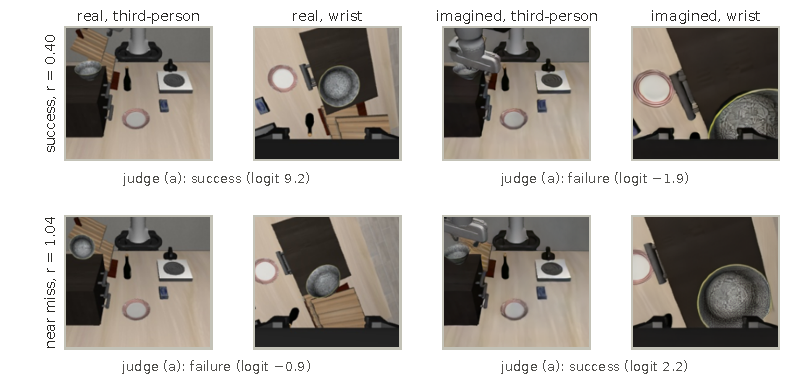
\includegraphics[width=0.82\linewidth]{figA_m2_frames.pdf}
\caption{M2, bowl on top of the cabinet, one imagined chunk: real and imagined frames after the lift, with judge (a)'s verdicts and logits. In imagination the arm stays lower, so the wrist view is closer to the bowl; the judge, trained on real frames, calls the success a failure and the near miss a success. The frames were regenerated for illustration and these two pairs were selected; on this task judge (a) labels 0.158 of imagined successes and 0.048 of imagined near misses as successful (Table~\ref{tab:m2tasks}).}
\label{fig:frames}
\end{figure}

\section{M3 Details}
\label{app:m3}

\textbf{World.} A two-dimensional pick task is rendered at 224 pixels by an object-centered side camera as an initial frame followed by four steps (move, descend and close, lift, lift). A grasp succeeds if the alignment error $e$ is below the object's half-width $w$, so $r=|e|/w$, and failures are deterministic.

\textbf{World model.} Frozen DINOv2 ViT-S/14 patch tokens are pooled $2\times2$ to 64 tokens and reduced to 64 dimensions per token by PCA. A pre-norm ViT predictor (four blocks, width 128, four heads, MLP width 512) takes the 64 frame tokens and an action token and predicts the next frame's tokens as a residual. It is trained by one-step teacher forcing with a mean-squared error on normalized tokens (AdamW, learning rate $3\times10^{-4}$, 300 warm-up steps, cosine decay, batch 256, 6,000 steps) on 30,000 episodes per seed, in which failures have $r\sim U[1,2)$ and occur at rate $p$ (about 900 unique failures at $p=0.03$). Imagination rolls the predictor four steps from the real first frame.

\textbf{Judge and policies.} The judge is an MLP on the real final frame's tokens, trained once and frozen (accuracy 1.000). The six policies draw $r$ from $|N(0,0.35^2)|$ (precise), $|N(0,0.6^2)|$ (good), $|N(0,0.9^2)|$ (medium), $|N(0,1.4^2)|$ (sloppy), or a 50/50 mixture of $U[0,0.8)$ with $U[1.5,2.0)$ (far-failer) or with $U[1.0,1.2)$ (near-failer), and are evaluated on 1,024 fixed scenes. The curve grid uses 49 values $r\in\{0.60,0.65,\dots,3.00\}$ on 128 scenes, with $r=3$ only on the 100 scenes narrow enough to fit.

\section{Additional Results}
\label{app:more}

\begin{table}[h]
\caption{Predictor capacity and representation in M3 ($p=0.03$, three seeds pooled; a descriptive analysis, not a planned test). AUROC of success against near misses on real frames, on imagined frames with the reference judge, and for a probe trained on imagined features; NM and SM with the reference judge. For the two token variants the frame set, judge and grid were rebuilt in the new representation (judge accuracy 1.000).}
\label{tab:capacity}
\centering\small
\begin{tabular}{lccccc}
\toprule
Variant & real & imagined & probe & NM & SM \\
\midrule
\inputrows{tables/tab_capacity.tex}
\bottomrule
\end{tabular}
\end{table}

\begin{table}[h]
\caption{All M1 counterfactual cells with judge (a): validation and training-split trajectories, both error definitions and all horizons. Near: number of near misses. Floor: near misses judged successful on real frames. Imagined: share judged successful among successes, near misses and far misses. Success vs.\ near-miss AUROC on real frames, on imagined frames and for the imagined-feature probe, and the AUROC drops against near and far misses.}
\label{tab:m1cells}
\centering\scriptsize
\setlength{\tabcolsep}{3.4pt}
\begin{tabular}{lllrcccccccccc}
\toprule
 & & & & & \multicolumn{3}{c}{imagined, judged successful} & \multicolumn{3}{c}{AUROC success vs.\ near} & & \\
\cmidrule(lr){6-8}\cmidrule(lr){9-11}
Split & Def. & $H$ & near & floor & success & near & far & real & imagined & probe & $\dauc_{\rm near}$ & $\dauc_{\rm far}$ \\
\midrule
\inputrows{tables/tabF_m1_cells.tex}
\bottomrule
\end{tabular}
\end{table}

\begin{table}[h]
\caption{Ranking metrics on every policy set (FGRE, MMRV, Pearson correlation of imagined with real success, and $\tau_b$ among pairs within 0.05 in real success). The control set and the VLM judge are not part of the H2 tests.}
\label{tab:rank}
\centering\small
\begin{tabular}{lcccc}
\toprule
Policy set and judge & FGRE & MMRV & Pearson & $\tau_b$ \\
\midrule
\inputrows{tables/tabF_rank.tex}
\bottomrule
\end{tabular}
\end{table}

\textbf{Perception floor by error component (M1, $H=5$, environment's $r$).} Near misses dominated by the pusher's position, the block's position and its angle are judged successful on real frames at 0.106, 0.154 and 0.111, so the floor does not come mainly from the pusher-dominated cases.

\textbf{Where the training signal lies.} The share of frame-to-frame change (innovation energy) in real DINOv2 features that falls on each region is 0.189 for the T block, 0.084 for the pusher and 0.727 for the background in M1, and 0.166 for the object, 0.126 for the gripper and 0.709 for the background in M3. DINOv2 patch features mix context, so background patches change even where nothing moves. Raising the boundary patches to half of the weighted energy, remedy (v), left NM at 0.144 on M1 (reweighting: 0.143) and 0.201 on M3 (0.187).

\textbf{Auxiliary judge (b) on M1.} The latent goal-distance threshold judges 0.313 of near misses successful in imagination at $H=5$, but 0.242 already on real frames, so most of its apparent optimism is perceptual.

\section{Compute}
\label{app:compute}

M1 and M3 ran on one RTX A5000 (24 GB) shared with another project; the stages of this study occupied it for about 15 hours of wall-clock time. M2 ran on rented NVIDIA A40 GPUs (a pod-hour is one hour of a rented machine): setup and reproduction (1.4 pod-hours), judge preparation and Diffusion Policy training for the dropped M2 policy stage (9.6 pod-hours), and the main counterfactual run on eight GPUs (22.3 pod-hours), USD 20.27 in total. The PointMaze replication ran on one rented A40 (1.4 pod-hours, USD 0.83). Analyses ran on CPUs.

\section{Reproducibility}
\label{app:repro}

The anonymized supplementary material contains the code that was run, organized by stage; the redacted design document with all amendments and the run log (Appendix~\ref{app:prereg}); the stage reports; and every analysis file from which the numbers, figures and tables of this paper are produced. Two scripts rebuild all figures and generated tables from those files, and a third checks every number quoted in the text against them. Upstream code was used at fixed commits: DINO-WM (0a9492f), Diffusion Policy (5ba07ac), Cosmos Policy (18a2acc), the LIBERO environment from LeRobot \citep{cadene2026lerobot} (14fd6f0) and CureWM (8a7ee5d). Seeds and splits are listed in the design document. Raw counterfactual records of M2's preparation stage (about 15,000 files) are provided as a separate anonymized archive.

\end{document}
